\documentclass[]{tufte-book}

% ams
\usepackage{amssymb,amsmath}

\usepackage{ifxetex,ifluatex}
\usepackage{fixltx2e} % provides \textsubscript
\ifnum 0\ifxetex 1\fi\ifluatex 1\fi=0 % if pdftex
  \usepackage[T1]{fontenc}
  \usepackage[utf8]{inputenc}
\else % if luatex or xelatex
  \makeatletter
  \@ifpackageloaded{fontspec}{}{\usepackage{fontspec}}
  \makeatother
  \defaultfontfeatures{Ligatures=TeX,Scale=MatchLowercase}
  \makeatletter
  \@ifpackageloaded{soul}{
     \renewcommand\allcapsspacing[1]{{\addfontfeature{LetterSpace=15}#1}}
     \renewcommand\smallcapsspacing[1]{{\addfontfeature{LetterSpace=10}#1}}
   }{}
  \makeatother

\fi

% graphix
\usepackage{graphicx}
\setkeys{Gin}{width=\linewidth,totalheight=\textheight,keepaspectratio}

% booktabs
\usepackage{booktabs}

% url
\usepackage{url}

% hyperref
\usepackage{hyperref}

% units.
\usepackage{units}


\setcounter{secnumdepth}{2}

% citations
\usepackage{natbib}
\bibliographystyle{apalike}

% pandoc syntax highlighting
\usepackage{color}
\usepackage{fancyvrb}
\newcommand{\VerbBar}{|}
\newcommand{\VERB}{\Verb[commandchars=\\\{\}]}
\DefineVerbatimEnvironment{Highlighting}{Verbatim}{commandchars=\\\{\}}
% Add ',fontsize=\small' for more characters per line
\newenvironment{Shaded}{}{}
\newcommand{\AlertTok}[1]{\textcolor[rgb]{1.00,0.00,0.00}{\textbf{#1}}}
\newcommand{\AnnotationTok}[1]{\textcolor[rgb]{0.38,0.63,0.69}{\textbf{\textit{#1}}}}
\newcommand{\AttributeTok}[1]{\textcolor[rgb]{0.49,0.56,0.16}{#1}}
\newcommand{\BaseNTok}[1]{\textcolor[rgb]{0.25,0.63,0.44}{#1}}
\newcommand{\BuiltInTok}[1]{#1}
\newcommand{\CharTok}[1]{\textcolor[rgb]{0.25,0.44,0.63}{#1}}
\newcommand{\CommentTok}[1]{\textcolor[rgb]{0.38,0.63,0.69}{\textit{#1}}}
\newcommand{\CommentVarTok}[1]{\textcolor[rgb]{0.38,0.63,0.69}{\textbf{\textit{#1}}}}
\newcommand{\ConstantTok}[1]{\textcolor[rgb]{0.53,0.00,0.00}{#1}}
\newcommand{\ControlFlowTok}[1]{\textcolor[rgb]{0.00,0.44,0.13}{\textbf{#1}}}
\newcommand{\DataTypeTok}[1]{\textcolor[rgb]{0.56,0.13,0.00}{#1}}
\newcommand{\DecValTok}[1]{\textcolor[rgb]{0.25,0.63,0.44}{#1}}
\newcommand{\DocumentationTok}[1]{\textcolor[rgb]{0.73,0.13,0.13}{\textit{#1}}}
\newcommand{\ErrorTok}[1]{\textcolor[rgb]{1.00,0.00,0.00}{\textbf{#1}}}
\newcommand{\ExtensionTok}[1]{#1}
\newcommand{\FloatTok}[1]{\textcolor[rgb]{0.25,0.63,0.44}{#1}}
\newcommand{\FunctionTok}[1]{\textcolor[rgb]{0.02,0.16,0.49}{#1}}
\newcommand{\ImportTok}[1]{#1}
\newcommand{\InformationTok}[1]{\textcolor[rgb]{0.38,0.63,0.69}{\textbf{\textit{#1}}}}
\newcommand{\KeywordTok}[1]{\textcolor[rgb]{0.00,0.44,0.13}{\textbf{#1}}}
\newcommand{\NormalTok}[1]{#1}
\newcommand{\OperatorTok}[1]{\textcolor[rgb]{0.40,0.40,0.40}{#1}}
\newcommand{\OtherTok}[1]{\textcolor[rgb]{0.00,0.44,0.13}{#1}}
\newcommand{\PreprocessorTok}[1]{\textcolor[rgb]{0.74,0.48,0.00}{#1}}
\newcommand{\RegionMarkerTok}[1]{#1}
\newcommand{\SpecialCharTok}[1]{\textcolor[rgb]{0.25,0.44,0.63}{#1}}
\newcommand{\SpecialStringTok}[1]{\textcolor[rgb]{0.73,0.40,0.53}{#1}}
\newcommand{\StringTok}[1]{\textcolor[rgb]{0.25,0.44,0.63}{#1}}
\newcommand{\VariableTok}[1]{\textcolor[rgb]{0.10,0.09,0.49}{#1}}
\newcommand{\VerbatimStringTok}[1]{\textcolor[rgb]{0.25,0.44,0.63}{#1}}
\newcommand{\WarningTok}[1]{\textcolor[rgb]{0.38,0.63,0.69}{\textbf{\textit{#1}}}}

% longtable
\usepackage{longtable,booktabs}

% multiplecol
\usepackage{multicol}

% strikeout
\usepackage[normalem]{ulem}

% morefloats
\usepackage{morefloats}


% tightlist macro required by pandoc >= 1.14
\providecommand{\tightlist}{%
  \setlength{\itemsep}{0pt}\setlength{\parskip}{0pt}}

% title / author / date
\title{现代科研指北}
\author{于淼}
\date{2019-03-13}

\usepackage{booktabs}
\usepackage{ctex}
%\setCJKmainfont{FangSong}
%\setCJKmonofont{KaiTi}
%\setCJKsansfont{SimHei}

\begin{document}

\maketitle



{
\setcounter{tocdepth}{1}
\tableofcontents
}

\chapter{前言}

才疏学浅,不知何为真,仅通少错之法,故不敢言南,仅指北。或曰:现代科研挖坑/跳坑指南

\hypertarget{intro}{%
\chapter{现代科研}\label{intro}}

\section{科学哲学沿革}

做科研一般都不讨论哲学,太多形而上的东西,说也说不清道也道不明还无法证伪。但懂一点科学哲学还是很有必要的,不然很容易研究着研究着就会觉得自己做的东西是垃圾,是谋生的工具,虽然从某个角度看也没错,但科学哲学无疑是应对这种心态最好的老鸭汤。

\subsection{古希腊}

哲学是爱智慧这个梗就不多说了,扯古希腊也显得俗套,反正有了古希腊人才有了理性跟逻辑的提法。古希腊前面的历史可理解成经验性知识的发展,知识多了就要有规律总结出来,逻辑和理性可看作用来生成规律的知识。其实哲学就是认识世界的知识,泰勒斯有一套,毕达哥拉斯有一套,赫拉克里特有一套\ldots{}\ldots{}大家能自圆其说就来一套,对不对另说,不服就辩论,赢了就是真理,输了就是谬误。如果说逻辑与理性出自于这些街头巷尾的辩论我一点也不会奇怪,因为两套理论对比,总得有两方都认可的法则才有结果,理性或许就是这种普遍性知识的产物。

不过辩论有诡辩这一说的,苏格拉底看不下去了就说你们这些人都觉得自己对,但有可能是不对的,反正我自知我无知(这句是我认可最有智慧含量的句子,还有一句:天下没有免费的午餐)。老苏不怎么关注解释万物,有点回归个人或社会的意思。到了柏拉图直接就理想国了,世界形物均为理型的影子。再到了亚里士多德就不怎么废话了,直接取消理型世界的存在,认为万物有因,这个因就是所有问题的因,寻找到最终因,真理就明了了。这货还不知道这个看法后来发展成第一推动问题,宗教界觉得只有全能的主有这能耐,就把亚里士多德的理论吸引到宗教哲学里去了。

同时,我们现在所提到的科学源于日本,可理解为分类的知识,而最早对人类知识体系分类的就是亚里士多德。他还很神奇的将自己的目的论揉到这个分类里去了,所以这个体系很完整,能解释的东西很多,所以后来几百年大家就都用了这个体系。其实这时候科学知识更适合分到亚里士多德所谓的自然哲学这个科目里,这个科目特指自然现象的规律及探索方法。这里需要注明的是数学更多是工具,数学化不一定就代表科学,另一个需要注意的是逻辑学,这货的三段论十分精彩,以至于要不是后来哥德尔横空出世,任谁也动不了根基。

\subsection{中世纪}

中世纪黑暗吗?如果看天气应该跟现在差不多,但这个黑暗的印象大致源于天主教对知识的垄断,而知识也反过来服务宗教,而宗教理性在一定程度上促进了我们对世界的认识,所以盲目对立宗教跟科学没必要,很多前期知识都是不少富有宗教热情的理性人士总结的。只不过知识很多种,科学在那年代连个独立的名字都没有,所以你看,牛顿写本书叫《自然哲学的数学原理》,跟现代意义上的科学没啥关系,所以你管他信仰什么呢。这个时候,科学知识跟形而上学还是分不开,很多知识有严谨的数学形式但你无法证实,很多天文学知识就这德行,你去看看托勒密体系,圆环套圆环的也能解释现象,那哥白尼的日心说为什么就流行了呢?因为是真理?因为结构简单?还是因为他用了别人看不懂的语言写出来的?或者说反对者死绝了新理论就流行了?总之,没有实证的理论的流行不会是你想的那么简单,但一般来说,人们都喜欢简单且解释面广的理论,宗教也这样,毕竟美的东西都是上帝赐予的。在科学这个提法之前,用一套知识来解释世界是各代学者所向往的,才不管验证什么的,理性重于事实。

\subsection{1500年以后}

时间点不太好找,但历史的发展是伴随知识的增长的。大航海时代为人类的知识提供了一个海量来源,文艺复兴带来了人性的解放,宗教改革让生活走出了政教合一,总之,经验开始比逻辑更为人接受。最开始是欧洲大陆的理性说与英国的经验论的争执,争论核心在知识的构建是从理性出发还是从经验出发,这两种观点打架几百年,到了19世纪末大家都不争了。因为实证主义一统江湖认为从经验中提取逻辑,然后再证实就OK了。这时候科学哲学才独立出来,而观察式的经验也开始让位于实验式的事实,人们不满足于被动接受知识,开始主动去寻找真相。

\subsection{逻辑实证主义}

当人自己把握了主动权,原有的常识知识就要被逻辑重新检验,而无法检验的就划到形而上学这一类里留给做宗教神学的人去讨论。换言之,从柏拉图开始的将现实世界与理想世界的区分被打破了,原来的哲学家都醉心于构建理想世界而不关心现实生活,而逻辑实证主义则要求通过生活的事实来寻找真相。换句话,经验事实及逻辑推理被结合用在真理的探索上了。而经验事实的崛起则伴随着归纳法的崛起,事实成为知识的唯一来源,科学开始渗入并改造哲学方法论,这一转变真正让科学有了真理探寻的光环,一举扫清神秘主义与宗教束缚,直到今天还在深刻的影响着每一个科研工作者。

\subsection{否证主义}

但不久大家发现不对头,因为归纳法不如演绎法严格,得到的结论有局限性,不够严谨。这时候波普就说了,演绎法靠谱!大家都提假说,然后验证它,出现反例就把假说否了,不能否证就不科学,这就是证伪。一时间大家都接受了,神马佛洛依德,历史唯物主义都因为自洽但不能证伪给踹出科学圈了。

不久又有人感觉不对了,一方面演绎法很难产生新知识,另一方面貌似假说是无穷无尽了。证实比较费事,证伪容易但很多理论就垮了。为了调和这个矛盾,否证主义给出的答案是演绎法虽不能产生新知识,但假说的产生不是无缘无故的,而知识的进步应该通过大胆猜想的确证与谨慎猜想的否证来完成,一个推翻的理论必然联系着新理论的提出,这时不断发展的,而科学的任务就是处理进步问题而非回答真理问题。形而上学也并不完全被排斥了,因为假说的提出有时就是没有事实证据的。进一步讲,波普尔将世界分成世界1,也就是物理世界,世界2,也就是精神世界,然后又分了个世界3,也就是客观知识世界。这种三分法其实是将柏拉图的理型世界进化了,同时也留下了世界2的个人空间。每个世界都在进化,这就是科学发展的轨迹。一口吃不成胖子,我们就去试错吧!猜想与批判这一否证主义的核心思想也是当下科研中比较闪光与巧妙的实验设计动机来源。

\subsection{历史主义}

前面那些理论的提出者大都数理化出身,推理证明构建系统很在行,但没案例不成啊,得解释得了现象啊。其中一些人翻了翻了史书,发现很多发现不是通过证伪得到认可的,也不是建立在大量归纳的基础上,而是具有``历史性''。也就是逻辑不怎么灵光,然后他们就说咱以史为鉴吧!拉卡托斯就搞出了个硬核软核的理论,大意说一个理论是有生命力的,硬核部分无须质疑,有保护带,一时半会死不了。需要缝缝补补的是外围软核,什么时候硬核也不行了,就退出历史舞台了。这个解释保全了科学理论体系,也就是堵了民科的路,要知道民科最喜欢证伪,一个错误就否了整体,现在拉卡托斯说不成,得慢慢来,有历史的。

不久又有人感觉不对了,我怎么知道现在的硬核到底对不对?拉卡托斯这时就呵呵了,交给历史评价吧!库恩在这个背景下提出了范式,他本身有较强的历史功底,手头案例多,所以有了科学共同体这个说法。大意就是一个时代的真理主流说了算,这伙人挂了而接任的更多采取了另一种解释现象更多的理论,那这个理论就上位了,就革命完成了。前面那个时期比较压抑就叫前科学,后面上位了就是常规科学。之后又有新现象解释不了了就有了危机,这时候新理论又出现了,再搞一次革命就OK了。范式是来区别前科学与常规科学的,范式通常是一套当前时代科学共同体所使用的理论体系,而这个理论体系要比之前的更能解释更多的问题也更严格。这理论比拉卡托斯那一套通俗易懂,那年代搞政治的一看有革命二字纷纷表示深有体会,大力推广之,所以范式着实火了好一段时间。

库恩的范式革命是格式塔式的转换,历史上一共也没发生几次,真正有益的是他对范式定义时要求要有自称科学的学科要有自己的理论体系与假设且对现实世界产生作用,这个理论自身并不要求科学家的态度是客观的,但范式自身要是客观的。这时候,大家都不愿搭理真理性这茬了,因为都清楚对错问题是历史性的。同时范式也把形而上学彻底请回到科学体系中了并认为对科学的发展是有益的,要知道波普尔虽然不拒斥形而上学但本质还是批判形而上学的。所以历史主义的强调使得真理相对化。

\subsection{无政府主义}

事实上你沿着这个思路走下去发现貌似科学发展跟三国演义差不多,不在于对不对而在于认可的多不多,有没有跟你闹革命的。当然因为实证主义的余威,理性与逻辑在科学研究中是绕不开的。这时候来了个更霸气的费耶阿本德,一拍桌子,科学跟别的知识没啥区别,不能特殊对待。 后来流传到世上的就是那句 anything goes ,很多人认为这货终结了科学哲学的发展。从20世纪初到六七十年代这个学科就完蛋了,这就是科学哲学的学科危机。

\subsection{实用主义}

逻辑委实打不过历史,原来那些搞科学哲学研究的还没死就没饭碗了,生存是硬道理。他们发挥了科学共同体的作用,把费耶阿本德斥为异类、后现代。但他说的话又绕不过去,这时候蒯茵跳出来说科学哲学还要发展,不能anything goes,科学不科学总得有个标准。美国人想来想去想到了有用两个字,然后大家纷纷鼓掌。理性,历史都打不过生存这个命题。有用是硬道理,有用解释一切,然后就没有然后了。

\subsection{其他}

除此之外,由于逻辑讲求语义明确而严格,但要是日常交流用一堆符号估计谁也受不了,所以科学哲学也在语义学方面继续发展。英国人的经验论也促进了新实验主义与主观贝叶斯学派的发展,慢慢地科学哲学也开始接受一些非实在论的观点,而科学实在论是穿插在上述命题中的。

科学哲学从实证主义发展到今天,被各种新命题与发现折腾的够呛,从里面提一个片段就可以看到很多,科学是什么?它跟哲学啥关系?又对哲学发展有什么样的影响?总之,我们没有停下探索真理的脚步,答案在哪里也毫无头绪,只要不满足于现状,知识就存在进步的可能,同时须知人生苦短,自知无知是很重要的。

就科研本身而言,最开始属于观察现象然后总结规律的经验方式,后来慢慢形成学科体系与知识框架来设计实验预测解释事实,现在其实更多是逻辑与经验的混合来解决科学问题。也就是说,学科知识是基础,但问题总出在前沿也就是知识覆盖不到或部分覆盖的地方,经验论与唯理论的斗争时常出现,单纯看经验或者说观察与实验会推动问题的解决,但有时候也推不动:很多规律不一定经得起检验,还有很多规律需要的限定条件太多进而导致应用上矫枉过正,还有些学科提出规律本身产生的反馈会导致规律失效\ldots{}

\section{科学知识的五个层次}

\subsection{背景组}

高中毕业水平。不论你学的文还是理,知识一般侧重原理或事实本身,或者说学到的是通识,例如地球是圆的、力学有三大定律、元素周期表是按什么排的\ldots{}这类知识其实就算老师不教,你看看《十万个为什么》什么的也大概能知道。

一般而言,科普主要面向知识背景是高中组的,因为绝大多数人不进行科研,就算进行科研其很多科学背景知识也是高中的,因为你大学可能学了某个学科,但另外的学科最理想也是停留在高中阶段。但这部分知识基本不用科普,或者说包含在更广泛的知识普及中就好了,需要思考推理的部分不多,主要是了解事实,形成背景概念。

\subsection{已知的已知组}

大学毕业水平。主要指专业知识,例如pm2.5是怎么回事?行星间距离如何测量?端粒长度跟寿命关系\ldots{}这个是社会大多数人科学背景知识的上限,也是职业化的下限。如果继续深究,基本就是做这一行的才了解,需要经验。目前这个层次的科学知识几乎可以被维基百科覆盖。如果你本科是理工学科,那么拿到学士学位就表明你已经掌握了这部分内容。这部分知识一般有自己的学科框架跟体系,但学科间壁垒明显,如果知识是构建在经验上的那么很有可能被机器超越而失业。

\subsection{已知的未知组}

这部分的知识是从已知走向未知,知识都是比较前沿的,很可能被后续结果推翻掉。所以这部分内容是需要不断研究的,但就研究思想层次看,其实即使一线科研工作者自己可能都比较迷糊,大部分人是站在前人基础上往前推进,前人的研究结论容易保存,但思想可能早就消散了。这阶段的知识因为开始走向应用所以学科间开始互通。科研人员的知识水平基本是这个层次的,知道前沿在哪里但还在探索。统计学也是这个阶段常用手段,但需要使用者理解方法本质,人工智能可作为研究方法但无法职业替代,因为探索性的思路还得人来启发。

\subsection{未知的已知组}

这个类别文章侧重于整合已有知识进行创新得到的新知识,基本上只有经验很丰富的人才能站到一定高度上理解一个学科。此时谈思想谈逻辑之外要整合学科历史,把发展沿革搞清楚。学科间知识高度互通,只有有洞见的科研人员才能掌握,统计学或人工智能在这个层次知识的失灵,只能摸着石头过河。

\subsection{未知的未知组}

这个组就是天花板了,或者走向科幻了。不过我觉得哪怕是科幻也是要读的,因为你可以体会其中思考的乐趣,当然知识背景设定就不要管了。这个组需要你能构建出一个逻辑自洽且符合现实的知识理论体系,其实就是形而上的东西了。我不认为现实世界中可以找出这样的人,但小说中是可以虚构出来的。

\section{知识体系的时间构建}

除了基于已知未知这种简单的面向科研划分方法,个人知识还需要一个时间与逻辑上的构建,这样可以自洽于其他非科研知识,毕竟科研是有噪音边界的,但知识却不一定有。

《四库全书》采用了经史子集的划分方法,内在逻辑是把经典的普世价值、过往的经验事实、学科知识与个人文集进行了区分,这样我们可以很容易找到知识的可靠性与归属。个人知识也可以分为形而上的观点理论与形而下的事实经验来区分,日常所见都是事实,前人所见则为历史,幻想与虚构的故事也是未来的存在,所以一个基础的形而下知识体系要有个人经验与历史,侧重对事实的准确描述,而关于未来则可单独开列,因为这类事实并不存在但不妨碍有思考的乐趣。至于形而上的东西,没必要确立经典,要按照逻辑自洽的原则去整理,包括有证据有逻辑的强理论;有逻辑无证据或弱证据的观点及个人经验;如果仅有证据没有观点,可移到形而下部分;仅有逻辑的理论是很危险的,若是科幻小说还值得看,否则不要随意吸收,因为这部分有可能指导改变世界,但尚属于探索,如果你不打算从政或成为企业家,可参考,但如果打算,就要考验个人决策能力了。科学探索恰恰可能也在这个地方,所以得学会用从观察与实验中提炼知识的能力,至于是否改变世界,那是你的自由。

简单说就是你可以创建一个笔记系统来整合你的知识:形而下的基础数据与案例库、历史沿革及信息检索方法与形而上的理论观点库,区分强理论与弱理论并学会总结理论。要学会把新信息整合到这个知识体系中去并持续整合,形成完整独立的知识库,这样就不容易被新思想所迷惑,总能找到位置。

\hypertarget{view}{%
\chapter{科研现状概览}\label{view}}

\section{问题为导向}

现代科研隶属于现代政治经济系统,满足社会的需求是其存在的基础,至于是否满足个人兴趣爱好与远大理想,可认为是副产品。当然,这是从社会层面说,具体到个人千差万别。

首先,我们要了解现代社会运行的基本模式,其中陌生人大尺度分工协作是现代社会最突出的特色。社会,简单说就是一群人而不是一个人生存的行为与知识模式集合。相比宗族或家庭为单位的原始聚居,古代与近代社会的发展不断突破着人们行为与知识范围的地理与血缘限制。

在原始聚居条件下,人们终生活动范围有限,语言隔阂等也限制了信息交流,好的生存模式很难传递到下一代或更远的地方,短暂的寿命基本都用在维持生存繁衍上了。当然,对原始部落的研究发现生活在其中的人并不比焦虑的现代人的快乐感受更少,但生活的自由度其实很有限(从另一方面讲,如果完全意识不到当今生活自由度可以改变其实也是一种内在幸福感,拥有更大自由度的人并不能完全体会到)。这种狩猎采集的原始聚居其实并不太需要共同的社会行为规则,但后来人们驯化了农作物与牲畜(其实很难讲谁驯化了谁,作物与牲畜也可能通过驯化更好的传播了基因),进而从流动走向了定居。

定居后的社会出现了更细致的分工,例如一个村落需要祭祀、防卫、生产、医疗等部门维持生存结构,这种分工有着自己的生命力,一旦产生会让整体受益,同时也会让这种结构加强。同样的,这种分工模式并不惟一,但如果两个定居的社会共同体产生利益矛盾,最后剩下来的总是一种更有利群体生存的模式,这个模式下的规则并无道德可言,或者说这就是社会道德的起源。这同时也是一个路径依赖的过程,总会带有一些副产品,很多时候我们就是通过副产品来回溯过去。如同对进化过程的研究一致,使用幸存者就是最好的或最合理的逻辑是不恰当的,我们需要通过回溯来发现一些制度历史上的合理性与偶然性,逻辑自洽并不代表历史真相,这点对科研认识也是很重要的。然而,这个阶段的社会政治经济体制依然很大程度被自然条件所控制,多数规则要么偏向农业社会,要么偏向海洋经济,人类的视野逐渐开阔,但基于血缘与地域的多样化依然可以保留,直到更追求效率的技术与体制规则进一步交互作用,孕育出近代工业社会。

近代工业社会将分工与效率推向了极致,影响的范围从多个国家推广到了全球。伴随而来的就是一套基本抛弃血缘关系与多样性的陌生人交流法则,地理限制被信息技术与交通技术打破,所有国家都会遵循同样的工业标准,语言也尽可能一致,法律也会去遵循共通的法则。科学研究在这个过程中起了很重要的作用,而工业化也不断向科研提出需求,此时科学研究从精英们的兴趣爱好变成了巨大的财富来源,每一次技术革新都服务了社会,而几乎所有的社会经济体都会拿出资金支持科研。务实一点的国家或企业会对工程学优先发展,而对自然科学的支持则颇有情怀意味,毕竟一旦经济下滑,最先拿不到钱的都是基础科研等见效慢的学科。这种社会整体的功利主义自产生之时就展示了巨大的生命力,甚至不断影响了社会中个体的决策行为。

时至今日,现代社会基本延续了工业社会对分工与效率的追求,但维持文化多样性与个体-社会相互关系的思考不断涌现。现代社会塑造了个体认知,个体认知却反过来反思现代社会的诸多问题例如民族主义的崛起、环境保护、气候变化、社会隔离与歧视、机会公平、人口老龄化、战争暴力、谣言传播、经济危机、金融危机、人工智能等。这些问题的根源有相当比例是社会政治经济体制的构建过程出现了漏洞,而今的科技发展把一些问题放大了,或者说这个系统需要打补丁了。毋庸置疑,科研对于现实问题的解决是一个靠谱的选择,其他选择例如宗教、回归原始生活更多的是一种消极的保守策略,选择那些方法并不会真的解决问题。这样如果给科研立块大牌坊,我想最好的题词就是从方法论层面解决社会问题。换言之,科研总是面向问题解决问题的一个社会分工,是一个职业,既不神圣也不低俗,从事这个职业的人总在用科学方法论解决实际问题,有时候也是揭示问题或为问题找一个解释。这个需求是根源,也就是说如果你科研自认为做的不错但跟现实脱节,那么即使留在象牙塔,也会面临自我认同与社会认同不协调的困境,需要你有额外的资源平衡。

放到经济视角下,这个职业也是有温饱小康问题的,也是一个利益集团,需要人代表到国会或人大去抢财政的分配,还要跟不同学科去抢所有的科研分配,充满了复杂的博弈过程,原来是陌生人之间,以后可能会发展到人跟机器或规则之间。这个职业有光环,但退却光环都是一个个为生计奔波劳碌的现代人,当然,不同人有着不同的生计标准。

\section{专业性与综合性的矛盾}

IT领域有一种职业叫做全栈工程师,指那种运用多领域知识完成产品的工作类型。最近发生的一些事让我越来越觉得科研领域也需要类似的概念,姑且就叫全栈科学家吧。

国内研究生培养的一个短板就是综合性不强,或者说科研民工,走出自己专业就不太敢想了,国外的研究生则对不懂的部分也有自信,最终能攒出一个结果,而这个结果可能要同时用到电子工程、材料、分析化学、机械及数据分析等多个方面的技术,即使没学过,他们也会通过学校找到合作的人。反观国内,研究生选课都很保守,不是自己以后研究领域的东西不选或直接让导师选,国外也会这样,但真遇到需要跨学科解决的问题从导师到学生都会想办法而不是觉得这东西不是我的领域就不研究了。打比方我设计一个算法,效果不错,但问题是别人不会用,那么就应该把算法打包成函数甚至设计一个简易图形界面让明白用途但不想理解算法的人用。但这个过程就不能靠分工了,得有人全流程都明白并进行整合,这种综合性有点类似工程师思维,甲方是同行,你得让同行解决实际问题而不是看你炫技术。基础学科肯定是有发展空间的,但目前基础学科要解决的问题已经都很像工程问题了,所以这类综合能力的问题化聚焦是实验学科研究生很重要的竞争力,痴迷于单一技术而看不到要实际解决的科学问题培养的只能是专家而不是科学家。

很多人觉得大学负责通识教育与精英教育,研究生要更多关注技能培训成为所谓专家,我觉得这可能是科研民工思想的源头。现状可能却是通识教育与精英教育从来都不如技能培训有吸引力,虽然可能潜力更高,这导致培养出的专家视野总是有局限性,需要在团队里合理配置才会提高解决问题的效率。例如想成为生物医药领域pi的研究生博后要在10年内搞出8篇一作才有戏,而H指数预测性很差,业界可拿这个数据到\href{https://peerj.com/articles/1262/}{学术圈}挖人。越来越长时间的专家培养是不可避免的趋势。

不过专家在团队里并不总是起正面效用,分工促进效率在面对可分解为具体步骤的行业或学科是好使的,但面对真实问题例如实验研究,实验者与数据处理者是不能脱节的。这里团队中指望两拨人放下成见平等交谈是很不现实的,因为占据理论高度的数据处理者或者说统计学家总会觉得做实验的是啥都不懂的。不过你不可能不湿鞋就过河,不了解实验具体操作就在那边对实验设计指指点点只会让实验者与统计学家的隔阂越来越大。所以我觉得解决实际问题需要培养全栈科学家,就是那种从采样到样品分析再到数据分析都有概念的科学家,即使以后实验可以外包也必须要进行所谓脏活的训练,数据科学家需要洗数据,全栈科学家可能连样品都要亲自采集,纸上谈兵绝对不行,养出一堆赵括天天跟你扯术语用的对不对完全就是浪费资源,全部开掉完全不影响进度,他们只是想通过凸显自己的专业性来找面子,根本就不打算解决问题。

现在的科研民工要有意识地训练自己成为全栈科学家,就算以后不做科研了,对实际问题解决的全流程理解也会让你很容易转行并与其他领域的人交流。更重要的是,这是所谓团队领导力的重要能力基础,几乎所有行业都对管理层培养有着基层轮岗的要求,公务员、医生、厨师、工程师还有律师等行业精英的训练过程都有着严格的全流程培训要求,搞空降或许会带来创新,但不了解步骤的空降几乎都是灾难。所以科研人员可以依赖专业人员,但心里要有问题解决的路线图与原理层的认识。不要过分依赖专家,他们都是为自己发声,只有你自己为你的项目负责,被专家牵着鼻子走对全栈科学家是一种耻辱,保证兼听则明就可以了。

专业的人喜欢谈差异与术语,解决问题的人更关注问题背后的共性。而统计学家也不要拿起实验设计不够随机与混杂因素工具变量啥的一堆术语去居高临下教育别人,这些问题要是都解决了一个t检验不就天下太平了,还需要统计学家做什么。扎根实际问题然后抽象出可测量的统计量,然后在模型中进行控制或考察,让结果具有可比性与重复性才是更重要的。我觉得统计学家不能固步自封,新技术一直在出现,新理念也一直在出现,自己不懂就去打击是很幼稚的行为。

虽然很多人批评文章数量不代表学科热度,但我觉得起码每篇论文都在解决一个科学问题,所以这里的比较就统一用文章数量。为了进一步简化评价,我们这里就用 pubmed 数据库作为例子,也就是说探索的是生物医药领域内不同研究领域的发展状况。方法也极为简单,就是关键词搜索。下面这个过程大家可以自行验证,其实用 web of science 更合理,但考虑到需要有对应权限我就不展示了,可自行探索。

首先先分析下具体的人。我自己追踪的学科内紧密相关研究一年发文量不超过100,也就是一个周一两篇的样子。这个知识更新频率应该是比较符合科研人员个体信息处理能力的。如果你关注的领域非常热,发文量很高,那么大概率你也会自主把文献查新的量通过关键词叠加来缩小到一周一两篇,一季度甚至一年出现一小领域综述的状态。而且这个量我觉得对大多数科研人员还是超载了,很多研究人员的课题非常精细,一年内同行发文量个位数,全世界也就几个课题组在做,那么此时应适当眼界放宽些,否则你的研究会被视野限制住。

当一个关键词年同行发文数量超过一百时,围绕这个关键词的全国性年会就会召开,也可能会拥有自己的专业期刊与学会,小型国际会议也可以组建了,例如纳米毒理学或持久性有机污染物。这个状态下的学科要么快速发展,要么快速衰退,全球相关课题组数量不会超过三位数,这类学科一年内如果频繁登上CNS,那么很可能进入指数增长期,但如果一年内一篇都没有,那消退也很快。如果低于这个量,那么关键词对应研究组可能还从属于某个大学科,属于大课题下的边缘课题,绝大多数退学的博士生都是挂在这类几乎看不到发展希望的项目上了。顺带一提,国内的杰青级评选的候选人至少要在国内是这个量级领域下的数一数二的人物,这样的领域整体看大概1000个左右。

当年同行发文量超过两千时,千人级国际性会议就能开,开的不错,行业内会出现多份期刊来吸纳不同层次的论文。而且我观察超过一千后的研究领域很少有萎缩的,但这是第一个停滞点,很多领域的规模上限就是两千。从人才角度看,国内在这个量级上数一数二的人物都是院士级的。这样的关键词例如纳米银、生物医药里的深度学习,这个量级如果能保持增长,那绝对会是学科热点,估计对应从业人员超过一万了,这类学科基本都有产业化的课题做支撑了。

年同行发文量在两千到一万的学科是非常多的,这是通常意义上的的科研 IP 例如代谢组学、精准医疗。这类研究你应该能从公众报道到听到了,全球有四位数的课题组,基本每所综合类大学都有至少一个人在从事相关研究。国家重点实验室基本都是在这个量级上构建的,企业也会有研发团队,且这个量级的实际需求已经有行业级支撑。

超过一万的关键词都可以称得上前沿或热点学科并且已经有能力渗透到其他学科了,例如纳米颗粒、基因组学、分析化学、睡眠、衰老等。每天科技新闻都会有相关报道,是CNS的常客。相关创业公司会受到科技类风投的重点关注。然而这里会遇到第二个停滞点,实际上这个量级的研究已经是此消彼长的发文量了,相互之间会有学科级资源分配问题,在国家层面会出政策来扶植这个量级学科的成长,当然如果财政有限,拿来支持的资源必然是其他学科抽的。这个级别是可能萎缩的,例如同位素研究在上世纪六七十年代曾经超过一万,但现在稳定在四五千的体量,这就是撞了停滞点了。

然而,还有一些顶级 IP 。生物医药科研里的顶级 IP 是细胞,最近三年年发文量稳定在不到27万的样子。然后是癌症,这个关键词最近三年基本稳定在17万。研究血液的在15年达到顶峰,发文量14万。脑类相关研究在17年见顶,不到8万的发文量。另一种热点疾病的是心脑血管疾病,在16年达到顶峰,大概不到7万的年发文量。有两点体会:

\begin{verbatim}
顶级IP一般要发文量超过5万,但似乎不会超过30万
很多顶级IP在14年之后停止了增长,或者稳定,或者干脆下降
\end{verbatim}

这些顶级 IP 而且几乎每一个都有一堆下属子学科,子学科的国际会议都能达到几千人级别。这些关键词几乎都配备国家实验室或研究所,数量每个国家也就十几个。这类学科已经不是渗透其他学科发展了,更多是引导性发展,这个领域出现的方法学进步会直接超越其他领域,也能吸引到很多超精英,带动整体进步。诺奖应该就是这个量级关键词上的进步的后果。

不过顶级 IP 在14年后的相对停滞是个值得关注的现象,我怀疑单一关键词存在一个体系上的发文上限,可能是经费、可能是人口、可能是整体教育水平、可能是技术限制、可能是资源相对竞争、也可能是难度。总之,数据就在那里,值得思考的东西很多。

这里我简单分个级(按幽游白书的分级方法):

\begin{verbatim}
S级 年同行发文量超过5万的关键词领域,疑似有停滞点
A级 年同行发文量1万到5万的关键词领域,有停滞点
B级 年同行发文量2千到1万的关键词领域,有停滞点
C级 年同行发文量100到2千的关键词领域
D级及以下 年同行发文量100以下的关键词领域
\end{verbatim}

这个应该就是科研人员的天梯系统了,研究在D级,关注到C级的研究动态,参与B级领域的会议,蹭A级的热点,然后远远看下S级开心就好。通过这种简单但可能不靠谱的分析,科研人员应该可以实现一个对自己的清楚定位,然后合理规划自己的视野,防止见树木不见森林,也防止迷失在过大的森林里。现在教学与技术手段已经足够发达了,培养一个全栈科学家可能并不比培养一个专家更困难。上世纪科研界花费了大量精力去构建术语体系与专业学科的墙,这个世纪我们该尝试打破这些意义不大的墙去解决一些复杂而现实的问题了。

\section{研究生教育的困境}

2018年国内研究生入学考试报名人数刷了新高,达到200多万,而这里面应届占一半多一些,报录比在缓慢降低。有一个很有意思的现象,报考研究生的人数并不是一直上升的,事实上,2007年、2013年都出现过报考高峰然后下一年回落的情况,回落可能跟当时经济形势上行有关,当社会岗位需求旺盛时,二三年的学位投资就可能是一笔很高的机会成本。但2016年起,研究生入学考试报名人数重新上升,这侧面体现了毕业生对就业的担忧。而且往届生与应届生报录人数同时增长,说明毕业生普遍认为学位比工作更有价值,或者说本科就业形势不佳。

我们再看看高考,中国高考报名人数在07-09这三年都突破了千万,此后人数稳定在九百四五十万的样子,录取则是在2016年达到巅峰的705万。对比高考录取人数与研究生录取人数就会发现高校中本科生规模已经见顶,但研究生规模持续增长,录取难度整体下降可能也是吸引考生报名的重要因素。

可以预计如果研究生持续扩招(推测2020年见顶),搞考研培训、出国培训、期刊校稿还有高校教职将出现最后的快速发展窗口,之后将进入稳定或衰落期。然而,这之前我们体会更明显的则会是更多关于研究生团体的讨论与新闻调查,我们的研究生教育发展可能还跟不上研究生团体扩大的速度,中间的差距是一头典型灰犀牛,潜伏巨大系统性危机。

从学生角度看,眼下的研究生报考热潮跟经济压力有关而跟科研兴趣没啥关系,所以很有可能出现学生自认打工仔的情况而在混日子等就业的情况,高校或研究所的心理辅导如果跟不上会出不少极端问题。从导师角度看,上个10年的高校扩张吸收了大量新导师,而持续增加的劳动力所需要的管理经验基本都比较欠缺,毕竟他们读研时周围没那么多学生,研究生无指导或指导过激情况会不断出现。我们会在近几年看到一系列因为研究生极端事件而采取的改进,但能否做到预防,就看高校研究所的领导团队是否有意识了。

研究生身份更像是一个容器,容器里面的是22-30岁的年轻人,都有着明确的导师学生关系,这个容器越大,微弱的声音就更可能汇聚成大的声响。这个群体的心理健康连同与之紧密相关的导师的心理健康都非常重要,这里面研究生群体是弱势群体,很多研究生对情绪调整可以说毫无头绪,这是成长的烦恼,但高校的象牙塔属性与导师制并不保证健康成长。社会里公司可以靠成熟持久的制度职场教做人,导师学生关系却永远只会是二到八年的临时身份,显然后者出问题概率更高。导师靠自觉来解决问题也并不容易,可以借鉴的经验基本就是个人成长经历,这玩意多半是个邻居孩子的故事,励志还行,并不能捕捉体会到当下研究生的真实感受。资源、机会、奖惩、社会整体就业压力都面临公平效率间的平衡管理,偏巧这玩意在日益侧重研究的高校研究所里是不教的。师生交流不畅会成为今后研究生教育问题重要来源。

读研的虽然是人口少数,但这部分人口掌握了相当的网络话语权。显而易见,未来几年我们社会里最有时间在网上发言的大学生研究生群体会持续走高,我们应该会看到更多对这个群体的讨论与新闻。事实上,千禧一代在制造话题上从来都是行家,他们伴随互联网技术崛起而成长,他们普遍教育程度的走高对整个社会,特别是舆论引导会产生巨大影响。如果你去回顾下这些年社会新闻的焦点,基本都能找到千禧一代的身影。他们在中国人口基数中比例很高,裹挟了上一个婴儿潮作为父母,可以说对很多经济形态例如网红经济、知识付费、新零售、消费升级、租房市场等提供了消费需求。他们的消费与网络话语权决定了新兴市场会听取他们的态度而不是大多数人的态度,而新闻媒体从来都是求新的。现代社会本质上就是知识精英的社会,因为现代社会的大厦只能通过各类专门知识来管理,单纯资本或人口不解决问题。

这是一个浪潮,浪潮的下一端是人口结构的变化,千禧一代可能是世界范围内最后的婴儿潮。眼下发生在非洲东南亚的那一拨可能有人口红利,但没有互联网同步发展的技术红利,如果不出现类似互联网的普惠技术,很多发展中国家事实上或者说政治上不存在多大的发展空间。所有问题都可能是时代问题,这几年有,下几年就没了,但身处时代之中的人往往是最容易看不到问题的。

\section{毕业延期问题}

根据最近20年研究生招生情况可以看出,研究生人数比例 研究所跟高校比例大概在1:3,硕士的扩招力度是远高于博士的,但两者都在扩,20年前一共6万多,现在仅博士每年录取就有7万多,硕士则扩张了10倍有余,达到每年六七十万的录取人数。从研究生毕业状况看,伴随扩招,每年招生人数与毕业人数有相当的差距,但比较吊诡的是博士招生在增长而毕业人数却趋稳了,这基本暗示延期,特别是博士延期的常态化。从在读人数上看,研究生这个临时身份群体在不断扩大,这造成了前文所述的研究生导师矛盾的激化,除了扩招影响,另一个自然就是前面提到的延期问题。

从教育部公布的数据推算,基本上博士延期概率超过50\%,硕士延期概率是个位数,也就是说``没有延期毕业的硕士,没有按期毕业的博士''这句话没毛病,而且延期超过50\%的时间已经超过10年了。同时另一个现象也值得关注,那就是女性研究生的延期概率是普遍低于平均水平的,那么对应的男性研究生延期概率会更加惨不忍睹。

如果我们用在校生去除当年毕业生,会得到一个预估的毕业年限,结果显示博士需要6年多毕业而硕士也需要3年多毕业,硕士那个考虑到延期概率不高还可以接受,博士那个就有点反人类了,而且从近几年情况看这个毕业年限还在增加。其实答案很简单,就是扩招导致的人口在高校或研究机构的滞留,那么如何去除这个影响呢?考虑到博士硕士其实应该是2-4年内毕业,我们只要用当年录取的人数去对比2-4年后毕业的人数就可以了。考虑到博士毕业率应该低于硕士且硕士毕业率不应该超过100\%,应该是3年毕业的数据比较可信,这里我们会发现3年毕业率要远高于延期概率,这又是怎么回事?

这里就没数据支持了,但我想大多数研究生都听过硕博连读这个概念,其实如果三年毕业为真,那么硕博加起来应该是6年,而硕博连读应该是5年,如果博士延期是常态化的,那么我想这里面很大一部分比例是硕博连读。估计再过几年,考博的比率可能会更低而硕博6年将成为默认的学习年限。有打算硕士毕业出国读博的可以考虑下了,年限上其实吃亏不多而且国外会有老板没钱了逼着早点毕业的情况。

刚才说了研究生毕业的供给端,下面看看需求端也就是教职的变化。国内教职因为99年开始的扩招导致在21世纪的第一个5年大量的扩展教职,这样的后果就是有一个5年的教职年龄高峰,这个高峰占据了大量的教职。从数据上看,目前这个高峰年龄段在51-55岁,都算是当打之年,如果退休年龄没有明显推迟的话,那么在10-15年后应该可以看到一个因为退休高峰导致的教职空缺期。那么10到15年后谁博士毕业呢?大概是现在读中学的孩子。其实考虑硕博6年加本科4年,每个高校都有义务在学生刚接触高等教育或研究时给他们领先当前技术10年的教材与方法,否则学生10年前选了小灵通网络优化专业,博士毕业基本就只有转行了。

这里再看下性别问题,数据显示女性教职前期扩张的要更厉害,平均年龄也更低,大概要20年左右才能迎来退休高峰的教职空缺,如果校方固定当前男女比,那么其实对有更低概率延期的女性并没有什么优势。

教职中教授的年龄分布状况也很有意思,结果显示教授平均年龄会大一点,当前教授主流是51-55岁,反推下基本是刚改革开放后上的大学,经历应该挺丰富的。我们再看下副教授的情况。可以看出副教授整体要比教授年轻10岁,大概90年前后上大学,46-50岁这个年龄段人数基本稳定,说明升教授基本就是前一个年龄段,从年龄分布上看35-45岁人多,不同代际间竞争会激烈些。

前面着重强调年龄分布可能带来的教职空缺,另一种空缺就是所谓扩张期或窗口期,我们不考虑退休,从年龄分布上看这一部分的人数似乎比较稳定。每年的教职数一直在提高,而是似乎斜率比较稳定。但是女性的教职数增长的回归斜率只有总数的1/3,也就是说每增长3个教职才会有一个是女性的,这说明教职市场存在一定的性别歧视。但这个问题不好直接下结论,因为辛普森悖论也是同样的语境。同时,教授与副教授教职增长的斜率低于总体,暗示了教职里存在的层级结构。总之,目前还算是一个稳定的窗口期,教职数不断增长,属于利好;但成长空间不算大,别忘了博士毕业生可是年年增长,所以以后熬年限是肯定不行的,31-35岁的副教授人数逐年下降,不是升迁(概率低)就是收紧了要求转而直接从海外引进人才,诸君努力吧。

我们都知道研究生学历在贬值,那么究竟贬到什么状况了呢?我计算了同年毕业的博士与硕士人数比例,很明显,硕士的贬值效果更强,博士相比之下反而在升值,女博士升值更高。当然,大前提是五十步笑百步,你懂的。基本的情况就是1个博士大概对应10个硕士,显然硕士作为一个学位扩的有点太猛了。后面的分析就不考虑硕士找教职了,基本没戏。

新增教职数这些年基本稳定在2万这个水平,博士毕业生大概超过5万,也就是说教职市场在今后可预期的时间里撑死也就能解决一半博士的就业,另外有一半肯定会转行。考虑到博士学位对硕士学位是升值的,估计非教职市场上应该挺容易就业的,当然看你干不干了。新教职里女性比例是低于人口比例的,但这二十年却一直在增长,同样在增长的则是博士毕业生中女性的比例,伴随这个趋势,教职里对女性的歧视似乎是要好于社会其他行业的。

\section{博士的就业问题}

2015年全国博士毕业生5.4万人,而去年大概到了6万人,按照很多人的说法,读到博士就应该去做学术,但我对这个问题做了一个费米估计,结果比较有意思,列出来供各位打算做学术的博士参考。

如果成为院士(中国科学院/中国工程院)算学术巅峰的话,那么院士的选拔可以看作到达顶峰的路径。选拔方法是什么呢?两年一次,一次总共大概150人,工程科学对半分,平均一年75人。

我们假定若干年后每年还是75人,因为两院院士总规模这么些年并未有很大规模的变化,就算加上文科一级教授也就是100这个数量级。

那么若干年后竞争这个数的人选平均看大概都是同年级的博士同学。目前每年全国土鳖博士毕业生6万多人,算上海归,同一年龄组大概7万人应该比较合理。

那么你看到了,你需要在同年级博士毕业生里成为千分之一左右的精英才算有希望成为院士级别的学者。这个似乎有点丧气,可能院士这个比较难搞,那么准院士的杰青呢?全国每年选拔200人为杰青,那么成功概率乐观估计是千分之三,杰青其实也很难了,我们再放宽到优青。全国每年选拔400人为优青,那么乐观估计成功几率大概是千分之五。即使我们大胆认为博士有一半不从事科研工作,几率翻倍成为优青也要是百里挑一。

也许你会说优青杰青比较遥远,那么教授或者正高不算遥远了吧,毕竟每个博士背后都有一个博导。那么全国博导能有多少呢,乐观估计6万,年龄分布从35岁到65岁,如果是均匀分布的话且保证65岁退休,那么每年能产生出2千正高岗位,除以当年大约7万的博士人数,这个比例不到百分之三。就算我把那些做学术但不培养博士的岗位算上,这个比例也不会超过5\%。硕士毕业生15年大概50万,说明副高大概最多也就这个数,每年也就1-2万岗位,也就是说大概20\%的博士最终能走到副高,其实这个比例也不算高,不过可以作为大多数人可以预想的目标。

你可能会说做学术要有一定理想,不能这么功利,说这话的有相当比例站着说话不腰疼。如果你已经走到教授研究员这个档次自然可以跟人谈理想,但坦白说现在的博导平均拿到学位都是20年前的事了,那个时候博士一年毕业7千多人,而现在博士毕业生数目翻了10倍,换句话在目前的晋升条件下你成为教授的概率大概是50\%,如果有一半不做学术,几乎可以肯定就是教授了。10年前一年博士毕业人数大概是现在的一半多,这意味着其晋升教授可能性也有十分之一,尚算合理。但10年后如果博士年毕业生达到10万,那么其成为教授将跟现在成为优青差不多难度,代际不平衡是十分严重的。不了解基础状况就把人往坑里带的后果挺严重的,自上而下,金字塔顶端人数就那么多,一味扩大底端几乎意味着大量博士要陷入无尽的博后循环之中去拉伸等级。

所以其实我挺理解很多劝博士毕业转行的看法的,那怕你手握博士学位,目前在国内想走到教授也是个p\textless{}0.05的事,大概20个人里有一个。考虑到一般博士同学同院系大概也就是20个人,如果学术水平不在前面,基本可以重新考虑下人生规划了,因为此时你选择科研就真的需要兴趣激发了,不然身边的落差会折磨你几十年。而且上面的估计有个严重的问题,那就是大量使用了均匀分布,但真实的情况却是极不均匀分布,你的师承关系跟毕业院校都会把这个分布搞得更加极端,而且后发者优势在科研里面非常常见,但前面的坑都满了你怎么让后发者上?

同时要注意,国内博士毕业生人数还在不断上升,一方面说明教职还是有空间的,另一方面则暗示了今后博士毕业生生存环境将会更加恶劣,竞争会更加激烈。同时,目前教职数目会逐渐趋稳,如果你没赶上新学科新方向的窗口期大爆发,基本就是始终要接纳这个竞争强度了,只会更强不会更弱。而且有些研究方向必然因为学科发展走向没落,没必要跟一伙老气横秋的人抱团取暖,该转方向就转,反正大家都没基础。

读博转行可能也是个好事,早点把青春奉献到知识洼地去才更能实现自己的价值,相比学术界科研,业界科研可能是一个很好的选择,毕竟能磕下博士学位,搞点别的也应该没啥问题。

同时,如果选择了科研道路也要知道上面的概率,当不成分子也可以先做分母,心态上说服自己静下心来做科研就OK了,乐在其中则何乐不为?切不可惶惶不可终日,空费时光。

\section{重要科研趋势}

\subsection{可重复性危机}

\begin{Shaded}
\begin{Highlighting}[]
\KeywordTok{library}\NormalTok{(scifigure)}
\NormalTok{exps <-}\StringTok{ }\KeywordTok{init_experiments}\NormalTok{(}\DecValTok{2}\NormalTok{)}
\NormalTok{exps[}\KeywordTok{c}\NormalTok{(}\StringTok{"analysis_plan"}\NormalTok{, }\StringTok{"data"}\NormalTok{), }\DecValTok{2}\NormalTok{] <-}\StringTok{ "unobserved"}
\NormalTok{exps[}\KeywordTok{c}\NormalTok{(}\StringTok{"experimenter"}\NormalTok{, }\StringTok{"analyst"}\NormalTok{, }\StringTok{"estimate"}\NormalTok{, }
    \StringTok{"claim"}\NormalTok{), }\DecValTok{2}\NormalTok{] <-}\StringTok{ "different"}
\NormalTok{exps[}\StringTok{"code"}\NormalTok{, }\DecValTok{2}\NormalTok{] <-}\StringTok{ "incorrect"}
\NormalTok{hide_stages =}\StringTok{ }\OtherTok{NULL}
\KeywordTok{sci_figure}\NormalTok{(exps)}
\end{Highlighting}
\end{Shaded}

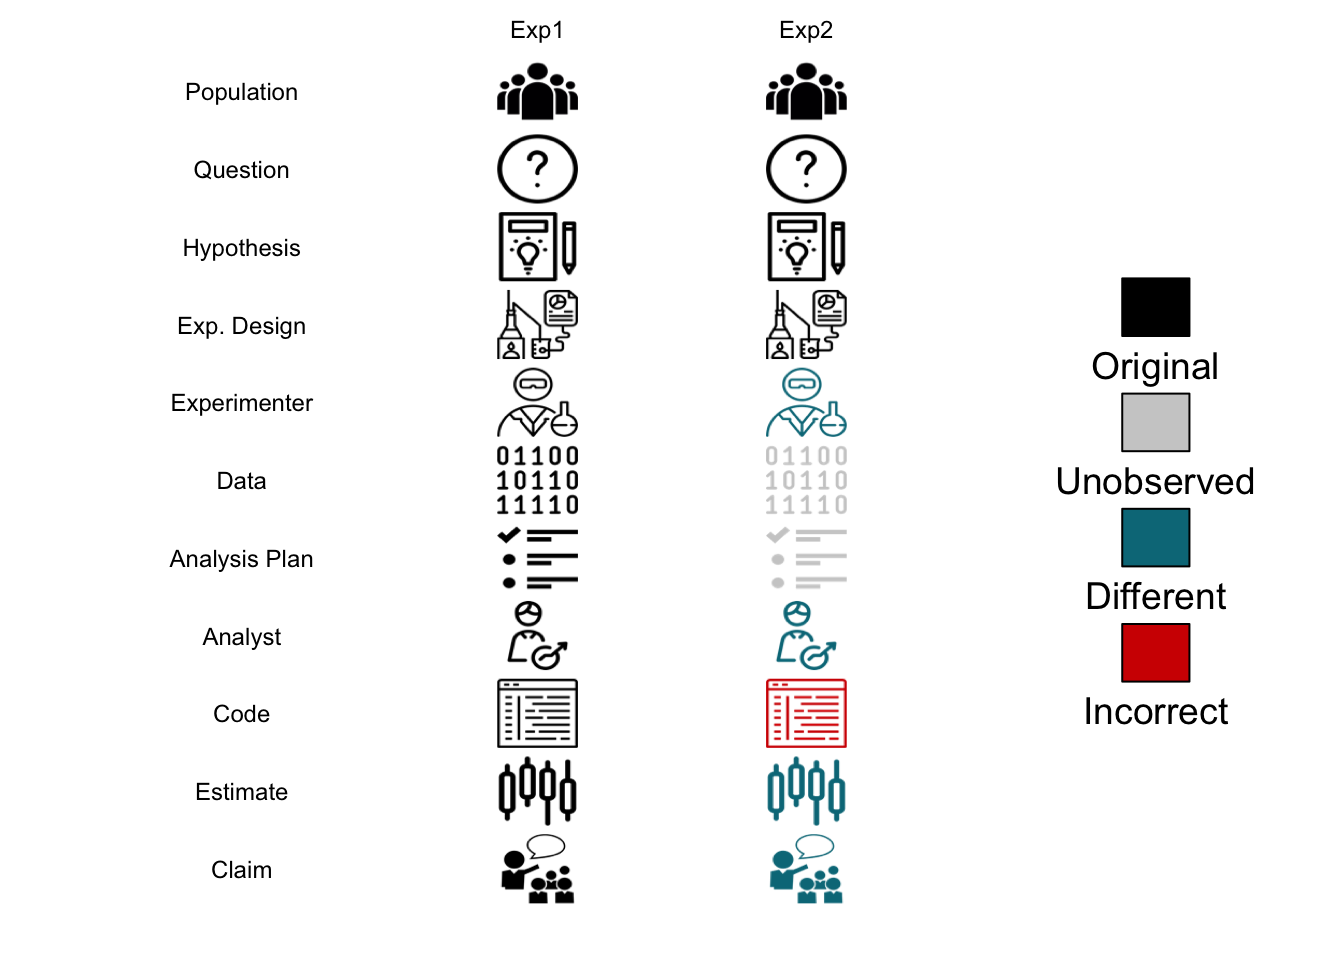
\includegraphics{sciguide_files/figure-latex/unnamed-chunk-1-1}

\begin{itemize}
\tightlist
\item
  \href{https://theoreticalecology.wordpress.com/2019/01/22/tree-species-richness-and-its-effects-on-productivity-neither-global-nor-consistent/}{预印本-博客-数据共享交流圈}
\end{itemize}

\subsection{军备竞赛}

\href{https://liorpachter.wordpress.com/2019/01/29/technologies-of-narcissism/}{预印本、开放获取期刊与社交网络互动是当前学术界的新潮流,不过也可能成为学术圈自恋的新战场,更高下载量与社交媒体转发评分有可能成为科研人员继SCI论文、影响因子与h指数后新的``优化''指数。}

\subsection{科学方法}

\begin{itemize}
\tightlist
\item
  基础学科信噪比高企与泛应用化
\item
  假设检验的困局
\item
  反馈对规律的影响:星座
\item
  平均律的终结
\item
  实际问题导向的基金流
\end{itemize}

\subsection{数据驱动的科研}

\begin{itemize}
\tightlist
\item
  多重检验问题与p值
\end{itemize}

疾病多个阶段都有指示物,根据不同阶段指示物进行综合判断,权重医生来定

频率

\begin{itemize}
\tightlist
\item
  概率是一个过程特性而不是结果
\item
  我不关心这个数可能是什么分布,只关心这个数具体是什么
\item
  \href{http://www.nature.com/news/one-size-fits-all-threshold-for-p-values-under-fire-1.22625}{p值这个问题,重要的不是把0.05降到0.005,通用阈值这个想法太偷懒,应该让研究人员充分理解p值实际意义与使用方法,毕竟在有些研究领域控制fdr后阈值实际比0.005低得多}
\item
  \href{https://www.nature.com/articles/d41586-017-07522-z}{\#nature\# nature就近年来的科研可重复性危机采访了五组科学家,分别从认知、NHST、FDR、数据共享与范式转化的角度进行了论述,当然别忘了到 Gelman 大人的博客上围观他的花式吐槽}
\end{itemize}

\subsection{假设检验问题}

\begin{itemize}
\tightlist
\item
  发现的价值不依赖p值,依赖效果大小与参数,进一步依赖样本量
\item
  p值常被认为随机生成的可能性,但混淆了P(D\textbar{}H0)与P(H0\textbar{}D), p值给的是前者,要想知道随机生成的概率,需要知道空假设是真的的概率
\item
  p值还被认为结果的可重复性,但重复性是统计功效的函数,跟p值无关,p值不能传达真实与否的信息
\item
  NHST用来评价空假设为真时观察概率,但多数情况不显著的结果是在研究假设而不是空假设下进行检验
\item
  统计功效很重要,跟样本数关系大
\item
  当样本数增大时,空检验总会被拒绝,因此当空假设为感兴趣的理论时,样本数与准确性会提高理论强度,但空假设不存在时,样本数与准确性提高只会弱化理论
\item
  发表歧视,科研文献不科学反应研究现状
\item
  基于p值还不如描述性统计
\item
  p值控制只考虑假阳性而不是假阴性
\item
  低功效研究会实际扩大研究的效果
\end{itemize}

John Myles White 系列

\begin{itemize}
\item
  隐藏多重检验,检测多个变量,留下显著的
\item
  NHST最大的问题在于解决问题的决策者与学术圈的认知不一样,研究人员的使用知识是不全面
\item
  对于个体而言可能还好,但对学术圈来说有时候是黑盒子
\item
  Cohen的国会议员例子,空假设是某人是美国人,备择假设是非美国人。我们知道某人是国会议员的概率是百万分之二,空假设里很难发生,备择假设里无法发生。空假设我们拒绝了某人是美国人,那么根据NHST,他不是美国人。但问题是议员一定要是美国人,在此类问题里,NHST永远无法认定稀有事件,也就是功效永远不足,并会给出错误答案。稀有事件总会发生,NHST总会把此类事件当成显著,即使不那么稀有,例如小概率事件如果发生了,我们就可以拒绝了。
\item
  进行假设检验时,我们是在测定空假设成立时数据发生的概率,P(D\textbar{}H0),但我们真正关心的是P(H0\textbar{}D),也就是数据是否支持假设,但这需要贝叶斯定律来计算
\item
  p值被用在同时测定效果强度与不确定性上,特别是很小但是很精确的差异,这是测量的进步,但却是理论的噪音,这样需要置信区间
\item
  p值的应用领域正在从硬领域走向软领域,低垂果实已经没了
  Paul Meehl:
  The almost universal reliance on merely refuting the null hypothesis as the standard method for corroborating substantive theories in the soft areas is\ldots{} basically unsound.
\item
  NHST已经不能帮我们积累知识,考虑一个多元线性模型,我们只能在多元模型里得到参数,也就是有限检验,不能发现未知参数,但科学就是寻找未知;变量间的关系在数值改变后如何考察,正负关系如何预测,预测性无法实现
\item
  p值正在成为测量投资与努力而不是事实的标准,给定差异,我们总能找到足够的样本来发现这个差异,如果打算测量就报告测量,p值并不能增加知识
\item
  对策

\begin{verbatim}
  - 停止使用假设检验,回归理论
  - 报告描述性统计,置信区间,效应大小与参数
  - 如果用,报道功效
  - 学科学哲学与科技史
  - Meehl: We should treat the history of science as a scientific problem.
  - 学数学:Use mathematical models to understand and explain the phenomena of interest; do not force the phenomena to fit a readily available, generic mathematical model.
\end{verbatim}
\end{itemize}

\subsection{贝叶斯}

\begin{itemize}
\tightlist
\item
  概率来自数据,长期表现需要分开讨论
\item
  我不关心我没有做过的实验,只关心基于当前实验能让我对这个数的估计改变多少
\item
  置信区间与可信区间(Confidence interval Credibility intervals)
  
  \url{http://stats.stackexchange.com/questions/2272/whats-the-difference-between-a-confidence-interval-and-a-credible-interval}
\end{itemize}

不用p值不会有type 1 跟type 2 错误,但是会有type s跟type m问题,前者是正负标志,后者是数量级

p值对个体研究者有意义但对群体有害,因为群体不知道个体研究的细节与尝试过程,例如找20个x与y关系总能发现有相关的,但只报道这个结果会导致其他人无法重复

Bayesian

\begin{itemize}
\item
  多重比较里,p值是根据你比较数而不是理论决定的,这导致你的主观臆断决定了结果
\item
  置信区间也会受到实验意图的影响
\item
  无限假设下,p值阈值可以无限小,也就是让所有结果都不再显著
\item
  设想投硬币跟投票,如果1000次有535次正面或投给候选人A,NHST无法区别,但贝叶斯下前者无偏,后者领先
\item
  贝叶斯方差分析先假设分布,然后用数据更新分布,后验分布计算出来就同时有点估计跟方差估计,同时多重比较问题也不存在,但随机错误无法避免,此时参数估计方差大也能体现,后续研究可以使用这次的后验数据作为下次先验数据
\item
  效应估计中95\% HDI 95高密度区间,空假设为真也会有5\%次没有真值
\item
  ROPE 真实等价范围,如果HDI不在区间内,那么拒绝,如果覆盖接受
\item
  效应估计的另一个方法是比较模型,参数可以来自收敛到更大的分布,这样可以降低错误,同时有利于空假设而不是拒绝,覆盖零不意味拒绝,有分布支撑
\item
  存在模型比较后空模型占优但是参数HDI排除了空模型,这个情况由于两个模型的先验概率对结果是敏感的
\item
  三种重复性:假设模型仿真看结果;后验模型仿真看结果;后验模型仿真后验模型做先验假设看累计效果
\item
  贝叶斯与频率学派之争
\end{itemize}

\url{http://andrewgelman.com/2012/07/31/what-is-a-bayesian/}

\url{http://andrewgelman.com/2012/02/24/untangling-the-jeffreys-lindley-paradox/}

\url{http://andrewgelman.com/2014/01/16/22571/}

\url{https://en.wikipedia.org/wiki/Lindley's_paradox\#The_lack_of_an_actual_paradox}

\url{https://xianblog.wordpress.com/2014/02/04/posterior-predictive-p-values/}
- 可重复性问题
- 《思考,快与慢》中启动效应的问题 \url{https://replicationindex.wordpress.com/2017/02/02/reconstruction-of-a-train-wreck-how-priming-research-went-of-the-rails/}

\subsection{社交网络中的科研}

\begin{itemize}
\tightlist
\item
  多媒体 v.s. 文字
\item
  快速反馈交流
\item
  合作全球化与圈子化
\item
  跨学科研究中的囚徒困境
\end{itemize}

\subsection{摘樱桃}

\begin{itemize}
\tightlist
\item
  荟萃分析中的摘樱桃问题
  \url{https://deevybee.blogspot.com/2018/07/standing-on-shoulders-of-giants-or.html}
\end{itemize}

\hypertarget{thought}{%
\chapter{思维工具篇}\label{thought}}

\section{科学思维}

\subsection{规律的失效}

科学靠谱很大程度是规律性进行的保障,规律保证了可预测性,但其实很多规律恰恰说明在很多地方没有规律。

\subsection{哈森奇效应}

\hypertarget{-}{%
\subsection{观察研究的敌人-反馈}\label{-}}

\section{模型思维}

模型思维是一种一对多的思维方法,从相似的事实中提炼出逻辑规律,用规律来指导认知世界,这种思维的优势在于逻辑或者说理性起决策主导参考作用。当一个模型出错时,我们可以运用其他模型来研究某个事实,因为所有的模型都存在简化,所以知道模型越多越有利于理解世界里发生的事。模型都有自己的准确度与适用范围,一般而言,高准确度的模型适用范围比较精确且会形式化为公式,而低准确度模型类似万金油,无所不包但含义模糊。模型化思考是首先抽离出变量,然后确定变量间关系,最后运用逻辑推理来进行思考的过程。模型终点可能是循环的、平衡的、随机的与不确定的,要用概率角度而不是决定论去看结果。

模型主要有两种,一种是基于公式的,另一种则是基于单元的仿真模型,前者需要你清楚的了解模型机理,后者则需要假定单元的活动空间与行为方式,然后通过模型运转来了解整体变化。

\subsection{可编程}

可编程是计算机科学的核心概念,当一件事可编程时,我们就可以设计出相对的硬件与软件来自动化这个过程。对于科研人员,硬件方面一般较少涉及,软件编程却是日趋日常化。因此,我们有必要了解编程语言的一些基本概念与思想。

程序是编程的结果,一般包含一条或一组执行运算的指令,这里运算并不仅仅指数学运算,也包括所有可通过电子电路完成的运算。要实现一次运算,我们至少需要输入值、运算与输出值。运算至少要能实现数值运算、顺序执行、条件执行与循环。因此,如果你打算进行编程,你就需要通过计算机语言让计算机知道输入输出与运算过程。

计算机语言不同于日常交流的自然语言(虽然可以处理自然语言),其核心特质在于描述上的准确性。不论操作符、数据类型还是函数定义,不同的计算机语言都有自己的规范来确保人要求的抽象化与机器能听懂人的要求之间达到平衡。底层语言例如汇编语言机器非常容易懂,但人不容易将需求转化为汇编语言。高级语言需要编译成底层语言来执行,不过人相对容易将需求进行编程。这个编译过程会损失效率,所以一般学习的语言越容易,效率与准确性往往会受影响。

科研里一般用程序来处理数据,所以科研编程的语言选择往往是实现效率、处理方法与编程难度的平衡。一般来说,数据处理方法源于统计学知识,编程难度取决于学科现实问题的抽象模型而实现效率属于纯计算机科学问题,科研人员可根据自己知识背景进行选择。对于非计算机科学专业的科研人员,建议关注学科内主流编程语言,否则后期会有很多交流上的困难,或者一步到位实现程序的应用化,让用户在少量编程知识的背景下就可以应用。

学习编程语言一般首先要掌握变量类型、赋值、表达式语法、保留词、注释等基本概念,然后就是大量的交互式案例训练来熟悉用法。编程语言一般会自带 REPL (Read--Eval--Print Loop;读取-执行-打印循环) 程序,在这个程序下会识别该编程语言的语法与操作符,互动地输入输出数据与结果。在编写程序代码时,最基础的要求是搞清楚编程语言的优先级,例如括号\textgreater{}指数\textgreater{}乘除法\textgreater{}加减法,一般执行顺序是从左到右。

另一种使用编程语言的方式是通过独立程序实现特定功能来完成的,运行程序可以直接得到输出,人机互动是在应用层上的。 REPL 方式其实比较符合数据分析的需求,后一种方式则反映了软件工程,涉及了程序的设计、构架与封装。目前科研应用中侧重交互式数据分析而业界则更看重程序编写与功能实现,前者存在试错且探索为主,后者则更侧重目标。这个区别专业程序员或软件工程师经常体会不到,觉得用 REPL 的科研数据分析是初学者,不能算编程。但其实科研数据分析的核心就是计算与需求的互动,REPL 只是其中一种,将需求从REPL过度成程序也是很重要。

也就是说,交互式与独立程序之间往往还有一个中间态,可以是脚本,也可以是自定义函数。一段代码一般是以输入为始,以输出为终,中间有函数来处理数据。在固定模式的数据处理中,一个函数的输出往往可以是另一个函数的输入,将输入输出代码按顺序、条件、循环排好就可以产生一个新的组合函数。事实上很多高级语言就在逻辑上抽象出一些常用函数来方便程序员直接调用。

同时,为了实现具体的功能,函数的输入除了数据外还有一些参数,有些是经验值,有些则可能要来自于功能本身定义。在输出上,有些函数的输出可以返回数值,有的可能就是打印到屏幕上就结束了,根据实际需求来。此外,多数语言的函数内部变量是只在内部可生产或可调用的,内部没有就可能从当前环境里找,最好不要设计这样的程序。函数或脚本对数据分析最大的意义在于减少重复工作与理清分析思路,对于软件工程则属于搭建工程部件,无论如何都是件功在当代利在千秋的事。

如果程序设计有问题,编程语言也会有对应 debug 的过程,大多数情况下是编程者的需求与机器的执行不对应导致,可以从这里入手思考修改代码。常见的错误包括但不限于语法错误、语义错误与例外。

下面重点讨论下编程思维中一些常见现象与术语,侧重理解并最好通过联系来强化理解。

\begin{itemize}
\item
  条件分支:函数中出现需要对数据子分类进行不同运算时的设计,不同子分类用不同条件语句进行逻辑判断,例如数值求绝对值要先判断正负。
\item
  循环:同样的操作要对不同的可索引或满足特定条件的数据进行运算,这种情况要设计循环结构,例如按数据行/列求值。有些循环循环数是知道的,有些则要对数据运行结果进行判断,满足特定条件时可跳出或继续循环。
\item
  递归:比较特殊的条件与循环结构,当数据不满足某条件时就执行函数本身直到满足条件,例如求解斐波那契数列之和就可以设计递归结构循环执行本身直到数据可计算的起点。递归的效率一般不高,但递归结构有助于简化思考问题的步骤。
\item
  正则表达式:正则表达式是字符串处理时常用的模式识别工具,灵活使用正则表达式与条件分支可以有效处理真实数据中的混杂,强烈推荐\href{https://zh.wikipedia.org/zh-hans/\%E6\%AD\%A3\%E5\%88\%99\%E8\%A1\%A8\%E8\%BE\%BE\%E5\%BC\%8F}{学习}掌握。
\item
  数据结构:通常不同数据按照实际需求会有不同的格式,不同格式的数据处理方式会不一样,一般函数都会先验证数据结构,如果不能处理则返回错误。
\item
  数据表:常见的数据处理格式,一般不同行表示不同样品,不同列表示不同样品属性且数据类型一致,数据值可以是数值、字符或逻辑值但不能是数据表。由于数据处理算法大都基于数据表开发,这类格式数据比较容易找到现成的算法函数/库/扩展包来进行处理。
\item
  字典:很多程序语言支持字典,字典是一种对应关系,字典中的元素是键值-数值对,通过键值索引数值,也可以反查。数据表中搜索元素是按照数值索引顺序索引的,字典则可以用哈希表快速索引。字典可以在编程中用来构建基于输入的数据库,方便进一步查询。
\item
  列表:列表属于数据表与字典的泛化,列表元素可以是数据表或列表,因此列表的数据结构不是平行的而是具备层级,有的元素可以进一步展开。列表常用来表示一组关联概念且可以数值索引,例如在回归分析的返回值中,就会包括拟合值、回归系数、残差等数据表或数值。
\item
  类型:通常列表可被定义成一种新通用类型,算法可基于这个类型进行开发或泛化,例如当你调用画图程序时,其程序会首先判断你输入数据的类型,如果有对应方法则直接调用,没有则用通用方法或返回错误。有些语言中列表是不能直接操作的,这样设计就是为了防止类型不兼容而强制定义格式。
\end{itemize}

其他一些概念例如并行运算、云计算、单元测试、集成测试、GPU加速、功能模块化、环境容器化、接口调用、功能移植、数据库检索、前端设计、数据加密、移动端兼容等都很有了解的必要,但这是建立在牢靠的基础上的。一个简单的判断标准就是根据你的需求你会觉得存在某种设计,然后一搜索发现果然有这样的领域,从需求出发回到需求中去是编程思维的要诀,不要在屠龙之术上花费太多时间。

\begin{itemize}
\tightlist
\item
  \href{https://benlauwens.github.io/ThinkJulia.jl/latest/book.html}{参考资料}
\end{itemize}

\subsection{预测模型}

\subsection{仿真模型}

\section{统计思维}

\subsection{统计量}

\subsection{回归}

\subsection{概率}

\subsection{方差}

\section{最优化思维}

\subsection{梯度下降}

\begin{itemize}
\tightlist
\item
  EM 算法 \url{https://www.nature.com/articles/nbt1406}
\end{itemize}

\subsection{动态规划}

\begin{itemize}
\tightlist
\item
  动态规划 \url{https://www.nature.com/articles/nbt0704-909}
\end{itemize}

\section{估算法}

\subsection{费米估计}

\url{http://www.mathsisfun.com/numbers/estimation.html}

\url{http://teachersinstitute.yale.edu/nationalcurriculum/units/2008/5/08.05.06.x.html}

\hypertarget{exp}{%
\chapter{实验}\label{exp}}

\section{实验设计原则}

试验设计一般是面向高年级本科生与研究生开的课程,但讲的都比较抽象。什么随机化、均匀性什么的道理都明白,但真到科研里面基本还是要依赖查表与软件分析。也正是因为如此很多人都是照葫芦画瓢来做,软件告诉哪个好就用哪个,在这种情况下软件实际充当了水晶球,你信就是了。

《Statistics for experimenters》的第一章是值得所有试验学科人读一下的,因为George Box 在第一章里没有扯什么随机化、均匀性,而是聊了下认识论。开篇第一句就是``知识就是力量'',解决问题实际就是一个认识模型演进的过程。具体来说是一个归纳-演绎不断往复的过程,数据起了中介作用。例如下面这个认识过程:

(模型)每天都一样

(演绎)今天车会停在原位

(数据)车不在

(归纳)有人偷车

(模型)车丢了

(演绎)车不在原位

(数据)车又回来了

(归纳)有人偷了车还回来了

不得不说我还是头一回发现认知过程可以这样描述的,具体到试验,这个过程就成了(模型)想法 -\textgreater{}(演绎)实验设计 -\textgreater{}(数据)结果分析 -\textgreater{}(归纳)结论或新想法。这大概是试验设计能上升到的最高理论高度了。

好了,不扯了,这本书非常适合读,但并不适合练。因为作者虽然用了很多很直观的解释方法让读者明白原理,但并未涉及软件层面。当然,提供代码也是最近才开始在技术书籍中流行的,这本书描绘了一个清晰的试验设计与分析框架,而我下面说的是结合R的一些从问题视角的实战。

现实生活中需要试验设计的场景一般都是多因素多水平寻优问题,翻译成人话就是 \(y = f(x)\) 中,y代表了你期望最优的东西,x代表了会对y产生影响的自变量,如果你的问题可以抽象成 \(y = f(x)\),那就可以通过构建模型来解决。试验设计主要关心的是方差分析这个视角,简单说就是y的变异可以拆分成不同x之间的独立变异或交互作用的线性组合。通过方差分析可以找到对y影响最大的x或所有x的影响方式,了解了影响方式,寻优什么的就比较简单了。

一般而言,想找出多因素的最优组合,第一步是要确定哪些因素重要而哪些因素不重要,这是PB设计的应用场景。在不考虑交互作用的前提下,通过PB设计的表头进行两水平试验,然后进行方差分析并可视化就可以筛选出重要因素了。PB设计的试验次数一定是4的倍数,而且最大适合因子数会比试验次数少1。打个比方,我打算找出9个因素中哪个影响目标最大,那么我的试验次数至少选12,下面是个演示,这里我们使用 \texttt{FrF2}包:

\begin{Shaded}
\begin{Highlighting}[]
\KeywordTok{suppressMessages}\NormalTok{(}\KeywordTok{library}\NormalTok{(FrF2))}
\KeywordTok{pb}\NormalTok{(}\DecValTok{12}\NormalTok{, }\DataTypeTok{nfactors =} \DecValTok{9}\NormalTok{)}
\end{Highlighting}
\end{Shaded}

\begin{verbatim}
##     A  B  C  D  E  F  G  H  J
## 1   1 -1 -1 -1  1 -1  1  1 -1
## 2  -1  1  1  1 -1 -1 -1  1 -1
## 3  -1  1  1 -1  1  1  1 -1 -1
## 4   1  1 -1  1  1  1 -1 -1 -1
## 5  -1  1 -1  1  1 -1  1  1  1
## 6   1  1  1 -1 -1 -1  1 -1  1
## 7   1  1 -1 -1 -1  1 -1  1  1
## 8  -1 -1 -1 -1 -1 -1 -1 -1 -1
## 9   1 -1  1  1  1 -1 -1 -1  1
## 10 -1 -1 -1  1 -1  1  1 -1  1
## 11  1 -1  1  1 -1  1  1  1 -1
## 12 -1 -1  1 -1  1  1 -1  1  1
## class=design, type= pb
\end{verbatim}

这里面1与-1分别代表两个水平,当然试验设计牵扯到分辨率问题,可以理解为对该试验设计的评价,分辨率高,能区分的影响就更细致,可以用\texttt{FrF2}包中的\texttt{GR}函数来计算。需要注意的是,\texttt{FrF2}包也可以用 \texttt{FrF2} 函数来进行两水平试验设计,这里是分辨率高时是可以考察交互作用的。

那么当你收集了数据,该如何分析呢?\texttt{FrF2}包实际继承了 \texttt{DoE.base} 包的S3对象类型,你只需要用 \texttt{add.response} 增加你的试验结果到设计出的S3对象上,然后就可以用方差分析或线性回归进行分析了。结果同样可以用\texttt{MEPlot}函数来进行可视化。当然,也可以用\texttt{halfnormal}函数来评价因子影响。

\begin{Shaded}
\begin{Highlighting}[]
\NormalTok{plan.annotated <-}\StringTok{ }\KeywordTok{pb}\NormalTok{(}\DecValTok{12}\NormalTok{, }\DataTypeTok{nfactors =} \DecValTok{9}\NormalTok{)}
\NormalTok{response <-}\StringTok{ }\KeywordTok{c}\NormalTok{(}\DecValTok{35}\NormalTok{, }\DecValTok{36}\NormalTok{, }\DecValTok{38}\NormalTok{, }\DecValTok{39}\NormalTok{, }\DecValTok{37}\NormalTok{, }\DecValTok{36}\NormalTok{, }\DecValTok{39}\NormalTok{, }\DecValTok{37}\NormalTok{, }
    \DecValTok{41}\NormalTok{, }\DecValTok{32}\NormalTok{, }\DecValTok{42}\NormalTok{, }\DecValTok{37}\NormalTok{)}
\NormalTok{plan.resp <-}\StringTok{ }\KeywordTok{add.response}\NormalTok{(plan.annotated, response)}
\KeywordTok{MEPlot}\NormalTok{(plan.resp, }\DataTypeTok{abbrev =} \DecValTok{5}\NormalTok{, }\DataTypeTok{cex.xax =} \FloatTok{1.6}\NormalTok{, }\DataTypeTok{cex.main =} \DecValTok{2}\NormalTok{)}
\end{Highlighting}
\end{Shaded}

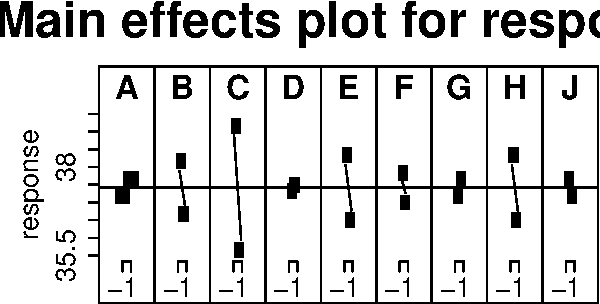
\includegraphics{sciguide_files/figure-latex/pba-1}

\begin{Shaded}
\begin{Highlighting}[]
\KeywordTok{summary}\NormalTok{(}\KeywordTok{lm}\NormalTok{(plan.resp))}
\end{Highlighting}
\end{Shaded}

\begin{verbatim}
## Number of observations used: 12 
## Formula:
## response ~ A + B + C + D + E + F + G + H + J
## 
## Call:
## lm.default(formula = fo, data = model.frame(fo, data = formula))
## 
## Residuals:
##       1       2       3       4       5 
## -0.1667  0.1667  1.6667  0.1667 -1.6667 
##       6       7       8       9      10 
##  1.6667  0.1667 -1.6667 -0.1667 -1.6667 
##      11      12 
##  1.6667 -0.1667 
## 
## Coefficients:
##             Estimate Std. Error t value
## (Intercept) 37.41667    0.83749  44.677
## A1          -1.25000    0.83749  -1.493
## B1          -0.41667    0.83749  -0.498
## C1          -1.08333    0.83749  -1.294
## D1          -0.75000    0.83749  -0.896
## E1           0.58333    0.83749   0.697
## F1           0.58333    0.83749   0.697
## G1          -0.08333    0.83749  -0.100
## H1          -0.41667    0.83749  -0.498
## J1          -0.91667    0.83749  -1.095
##             Pr(>|t|)    
## (Intercept) 0.000501 ***
## A1          0.274099    
## B1          0.668138    
## C1          0.325074    
## D1          0.465006    
## E1          0.558164    
## F1          0.558164    
## G1          0.929814    
## H1          0.668138    
## J1          0.387944    
## ---
## Signif. codes:  
##   0 '***' 0.001 '**' 0.01 '*' 0.05 '.' 0.1  ' ' 1
## 
## Residual standard error: 2.901 on 2 degrees of freedom
## Multiple R-squared:  0.7867, Adjusted R-squared:  -0.1732 
## F-statistic: 0.8196 on 9 and 2 DF,  p-value: 0.6603
\end{verbatim}

在这里PB设计实际上是一种预选法,如果结果显示某些变量影响显著,那么事实上就可以针对这些变量进行进一步的精细筛选,其余的变量可以直接固定为一个水平进行进一步设计。PB法在工业届用的比较多,但你应该想到了,如果只是进行变量选择,为啥不用随机森林或lasso?其实都可以,但这些方法不是设计而更多是数据分析通用方法,设计上除了最重要的随机性也是要考虑各因子贡献或者说重复数尽量平衡些的,否则会过分偏重某个因子,或者干脆配对或组成区组。像这样不做预设去设计对各个因子都公平,如果有预设或现实条件不允许,也可以裂区设计。

当选出重要因素时,下一步常见是正交试验或响应面分析,用来优选参数。正交表这玩意我在书中没找到,文献里用得多的也是亚洲人,老外统一用析因试验来进行考察。其实正交表的设计原理就是用尽量少的步骤遍历掉因子空间,这样进行一定次数试验就可以发现最优组合。R中的实现基本都在\texttt{DoE.base} 包里,这个包内置了一堆可以直接调用的正交表,可以根据需求进行查询。例如我有6个因素,水平数分别是2,3,3,2,2,6,然后我只打算做不超过54次试验,这时可以直接调用\texttt{show.oas}函数进行查询,给出的正交表随意选一个就可以继续。

\begin{Shaded}
\begin{Highlighting}[]
\KeywordTok{show.oas}\NormalTok{(}\DataTypeTok{nruns =} \KeywordTok{c}\NormalTok{(}\DecValTok{0}\NormalTok{, }\DecValTok{54}\NormalTok{), }\DataTypeTok{nlevels =} \KeywordTok{c}\NormalTok{(}\DecValTok{2}\NormalTok{, }\DecValTok{3}\NormalTok{, }\DecValTok{3}\NormalTok{, }
    \DecValTok{2}\NormalTok{, }\DecValTok{2}\NormalTok{, }\DecValTok{6}\NormalTok{), }\DataTypeTok{showmetrics =} \OtherTok{TRUE}\NormalTok{)}
\end{Highlighting}
\end{Shaded}

\begin{verbatim}
## no suitable  resolution IV or more  array found
## 5  orthogonal  arrays found
##                name nruns lineage   GR GRind
## 78 L36.2.13.3.2.6.1    36         3.00  3.00
## 81 L36.2.10.3.8.6.1    36         3.18  3.18
## 83  L36.2.9.3.4.6.2    36         3.00  3.00
## 87  L36.2.3.3.9.6.1    36         3.18  3.00
## 88  L36.2.3.3.2.6.3    36         3.00  3.00
##    regular SCones    A3    A4   A5    A6
## 78   FALSE      6  45.3 158.4  426  1010
## 81   FALSE      0 130.3 737.2 3063 11096
## 83   FALSE     17  82.3 338.2 1025  2828
## 87   FALSE     12  73.8 300.2  912  2404
## 88   FALSE     37  35.6  73.1  120   125
##         A7      A8
## 78  1753.2  2306.8
## 81 31380.8 68828.1
## 83  5507.5  7780.0
## 87  4354.2  5793.4
## 88    63.5    13.9
\end{verbatim}

这里我们选分辨率略高的\texttt{L36.2.10.3.8.6.1},从名字上看,这是一个36次试验表,可以包含10个两水平,8个三水平与1个六水平因子,这也是唯一一个分辨率高于3,可以排除交互作用的设计方法。这里我反复提到分辨率,实际上就是一种考察试验设计合理性的指标,分辨率3一般指只能区分没有交互作用的各因子贡献差异,高于3就可以区分一定的因子交互作用,可以用\texttt{GR}去计算一个广义分辨率并用\texttt{oa.design}来进一步优化这个设计,因为其实符合正交表只是众多选择的一个子集,不过根据优化方法的不同,优化时间也不太一样。

\begin{Shaded}
\begin{Highlighting}[]
\KeywordTok{oa.design}\NormalTok{(L36.}\DecValTok{2}\NormalTok{.}\DecValTok{10}\NormalTok{.}\DecValTok{3}\NormalTok{.}\DecValTok{8}\NormalTok{.}\FloatTok{6.1}\NormalTok{, }\DataTypeTok{nlevels =} \KeywordTok{c}\NormalTok{(}\DecValTok{2}\NormalTok{, }\DecValTok{3}\NormalTok{, }
    \DecValTok{3}\NormalTok{, }\DecValTok{2}\NormalTok{, }\DecValTok{2}\NormalTok{, }\DecValTok{6}\NormalTok{), }\DataTypeTok{columns =} \StringTok{"min34"}\NormalTok{)}
\end{Highlighting}
\end{Shaded}

\begin{verbatim}
##    A B C D E F
## 1  2 2 3 1 1 2
## 2  2 1 3 2 2 1
## 3  1 1 2 2 2 3
## 4  2 3 1 1 1 4
## 5  2 3 2 2 1 1
## 6  2 2 1 2 1 5
## 7  1 1 3 1 2 2
## 8  2 1 2 1 2 4
## 9  2 1 3 2 1 3
## 10 1 3 2 2 1 2
## 11 2 3 2 2 2 5
## 12 1 3 3 1 1 5
## 13 2 3 3 1 2 3
## 14 2 3 3 2 1 6
## 15 1 2 2 2 2 2
## 16 1 1 2 1 1 5
## 17 1 2 1 1 2 4
## 18 1 3 3 2 2 4
## 19 2 2 2 2 1 4
## 20 2 1 1 1 2 5
## 21 2 1 2 1 1 6
## 22 1 1 3 2 1 4
## 23 2 1 1 2 1 2
## 24 1 2 3 2 2 5
## 25 1 2 1 2 1 6
## 26 2 2 2 1 2 1
## 27 1 1 1 1 1 1
## 28 1 2 2 1 1 3
## 29 1 3 1 1 1 3
## 30 2 3 1 1 2 2
## 31 1 3 1 2 2 1
## 32 1 2 3 1 1 1
## 33 1 1 1 2 2 6
## 34 1 3 2 1 2 6
## 35 2 2 1 2 2 3
## 36 2 2 3 1 2 6
## class=design, type= oa
\end{verbatim}

使用这个函数你就不用费力去套正交表了,直接可以用输出的设计方案,记得要说明你的分辨率优化方案。如果你坚持套正交表,一定要理解如何去套,因为正交表的排列是很讲究的,特别是你要考虑交互作用的影响。如果一个表最多14个因子而你就设计了14个因子,那么分辨率不会超过3。正交设计的分析与前面PB设计是一致的,都是沿用添加响应,然后方差分析或线性分析随意来就是了,\texttt{DoE.base} 包为\texttt{design}这个对象类型设置了\texttt{lm}与\texttt{aov}方法。

在进行数据分析时,有时会遇到方差分析与线性回归的区别问题,打比方你用线性回归来做分析,会有审稿人问你lack of fit检验有没有做。这个检验实质上也是个F检验,用来衡量线性模型之外残差里分组变异与纯误差变异的比值,如果分组变异还是比较大,那么线性假设可能就不合理。

不过,目前试验设计结果分析更精细的会用响应面分析。顾名思义,响应面有点梯度下降迭代寻优的意思,而且如果是曲面通常考虑了二阶甚至更高阶的交互作用。在R中的实现是通过 \texttt{rsm} 包来进行的,这个包也是囊括了设计与分析两个部分,设计部分也有常见的 Box-Wilson Central Composite Designs 与Box-Behnken designs,分析部分自然还是基于\texttt{lm}的。同样,对于CCD设计,也提供了\texttt{ccd.pick}来选择好的设计,这里好自然意味着一些表征设计均衡的统计量。因为\texttt{rsm} 包小品文写的很清楚了,我就略过演示了。如果你面临多响应同步优化问题,那么\texttt{desirability}包考虑一下有没有,这个包其实是定义了一个多响应的联合满意度作为目标统计量,然后用响应面分析进行寻优,对于组学研究是有启发的。另外说个小八卦,狭义正交表也就是田口设计其实最初是两响应优化,只不过另一个响应是无法控制的噪音,田口搞了个信噪比来解决问题,熟悉了这套统计量构建策略,你也应该能做到根据实际情况构建指标体系。

其实试验设计分析是可以用所有符合\(y = f(x)\)的模型来操作的,说白了就是参数寻优。但试验设计更独特的点就在设计上,更广义地讲,A/B测试等纯计算试验也可以套用试验设计原理,这里要区分清楚设计与分析,设计不合理,分析会很头痛。如果再扩展些,观察研究的试验设计相比控制实验更关注配对或策略抽样。总之试验设计并不是什么水晶球,其原则从来都很清楚,只是后来流派出的太多,术语也越来越晦涩。然后你就会在网上看到哪个软件能做哪个分析的讨论了,其实这情况在工科可能更严重些,例如混料配比的\href{https://support.minitab.com/zh-cn/minitab/18/help-and-how-to/modeling-statistics/doe/supporting-topics/mixture-designs/what-is-a-mixture-design/}{三角坐标系设计}就完全是另一套,不过万变不离其宗,说白了还是个响应面分析。

\section{定性实验}

\section{定量实验}

\section{思想实验}

\begin{itemize}
\tightlist
\item
  \href{https://www.vox.com/technology/2016/6/23/12007694/elon-musk-simulation-cartoon}{人是否在仿真中}
\end{itemize}

\hypertarget{data}{%
\chapter{数据处理}\label{data}}

数据处理是科研中很重要的一环,同样的数据不同的人处理会得到不同的结论。事实只有一个,但解释可以有很多,数据处理方式本身就会对解释产生影响。这里重点讨论几个常见的数据处理问题。

\section{多重比较}

\begin{itemize}
\item
  多重比较问题 \url{https://www.nature.com/articles/nbt1209-1135}
\item
  Bretz, F., Hothorn, T., Westfall, P., 2010. Multiple Comparisons Using R. CRC Press.
  Gabriel, K.R., 1978. A Simple Method of Multiple Comparisons of Means. J. Am. Stat. Assoc. 73, 724. \url{https://doi.org/10.2307/2286265}
\item
  Gelman, A., Hill, J., Yajima, M., 2009. Why we (usually) don't have to worry about multiple comparisons. ArXiv09072478 Stat.
\item
  Plotting of multiple comparisons? {[}WWW Document{]}, n.d. URL \url{http://stackoverflow.com/questions/2286085/plotting-of-multiple-comparisons} (accessed 11.9.13).
\item
  Rafter, J.A., Abell, M.L., Braselton, J.P., 2002. Multiple comparison methods for means. Siam Rev.~44, 259--278.
  Stoline, M.R., Ury, H.K., 1979. Tables of the Studentized Maximum Modulus Distribution and an Application to Multiple Comparisons among Means. Technometrics 21, 87. \url{https://doi.org/10.2307/1268584}
\item
  \href{https://zh.wikipedia.org/wiki/\%E5\%A4\%9A\%E9\%87\%8D\%E6\%AF\%94\%E8\%BC\%83\%E8\%AC\%AC\%E8\%AA\%A4}{多重比较谬误}
\end{itemize}

\section{多重检验}

\begin{itemize}
\tightlist
\item
  p值
\end{itemize}

\section{线性模型}

\begin{itemize}
\tightlist
\item
  从lasso到岭回归,惩罚项在回归分析中的应用
\item
  截断回归与缺失值处理
\item
  线性混合模型
\item
  线性模型中非考察变量的判定与消除
\item
  分层模型 \url{https://www.nature.com/articles/nbt.1619}
\item
  线性判别分析与特征发现
\item
  logistic回归与剂量效应曲线
\item
  相关性分析与工具变量 \url{https://www.nature.com/articles/nbt0309-255}
\item
  偏最小二乘分析在结构效应关系研究中的应用
\end{itemize}

\section{模型}

\begin{itemize}
\item
  MCMC方法 \url{https://www.nature.com/articles/nbt1004-1315}
\item
  聚类与主成分分析 \url{https://www.nature.com/articles/nbt0308-303} \url{https://www.nature.com/articles/nbt1205-1499}
\item
  列联表分析与流行病学研究
\item
  人工神经网络与黑箱计算 \url{http://www.nature.com/doifinder/10.1038/nbt1386}
\item
  支持向量机的回归与分类 \url{https://www.nature.com/articles/nbt1206-1565}
\item
  从决策树到随机森林 \url{http://www.nature.com/doifinder/10.1038/nbt0908-1011}
\item
  经验贝叶斯与近似贝叶斯计算(ABC)及贝叶斯网络 \url{https://www.nature.com/articles/nbt0106-51}
  \url{https://www.nature.com/articles/nbt0806-959}
  \url{https://www.nature.com/articles/nbt0904-1177}
\item
  时间序列分析
\item
  结构方程模型
\end{itemize}

\section{可视化}

\section{重采样}

\begin{itemize}
\tightlist
\item
  bootstrap思想
\end{itemize}

\section{常见算法解析}

\hypertarget{lib}{%
\chapter{文献}\label{lib}}

\section{文献管理}

文献管理方面主要包括文献收集、整理、分析与追踪,目的是获取当前研究趋势。用认知过程阶段可以分成三个:从无到有、从有到精与从精到用,从无到有是指刚进入一个新领域时的状态,绝大多数研究生跟转行的科研人员都要通过这个阶段构建自己的文献知识库;从有到精指维护与整理与追踪新文献;从精到用阶段指文献知识库体系直接参与科研过程形成产出的过程。

\subsection{从无到有}

刚开展研究工作的第一步就是背景知识的了解,除非你研究生转行,一般本科阶段的学习应该已经掌握了学科基础,这个是共通的背景知识。基于此你要从教科书上相对确定的知识走向文献资料中相对不那么确定的知识,此时最好的开端是一本英文教材,一方面锻炼英文,另一方面英文教材的更新比国内要快(你大概率可以从图书馆借到,而且多数图书馆都有根据你需求订书的服务,不要浪费)。如果你精力足够,甚至可以联系作者问下是否可以翻译,这样一举多得,不过我没操作过,只是建议。另一个思路是通过 MOOCs 来系统学习,国内外很多高校放到网上的课程授课老师都属于接受新思想比较快的人,讲义也比较前沿,系统性比较高。还有一个不太通用的方法是阅读近些年的博士论文,其文献部分一般都是相关信息,不过能不能找到就不好说了。这个阶段一般要两三个月,不要心急,先把基础打好。前面掉的坑越多,后面跳坑就更有经验。

一般而言,一项学术成果要先发表,然后被综述评论,然后进入研究生课程讨论班,然后进入本科生课程讲义,最后才进入学科经典教材的更新。所以你可以倒着去走这个流程,越往后可能越不容易懂,但循序渐进总比一下读前沿论文被搞晕要好。有了相对前沿的教材或讲义作为知识框架,你的脑子里此时应该比较清楚导师让你做的东西或自己打算做的东西在学科中的定位,解决的是什么科学或工程问题,此时可以进行基于关键词检索的文献收集了。

一个良好的搜索返回的结果应该在10篇以内,首先要是综述,然后关键词检索方面建议学点逻辑运算符来过滤掉不相关信息,如果你上一阶段看的书是5年前更新的,那就只去关注最近5年的综述;如果你做的领域实在太新,那就把关键词信息的同义词跟近义词也加到搜索里;如果你能找到一篇写的特别好的综述或者有高人指点的论文,那是最高效的方法,可遇不可求。这10篇论文请按年为单位每1-2年选一篇综述去看,一月内读完,要求是精读,也就是论文里提到的研究都加到你的文献库里并阅读细节,同时可参考综述章节对文献库进行分组。一定要做笔记,而且要进行结构化的笔记或思维导图,这个阶段时间可能比较长也比较累,成果是当你去听系里的报告时,你大概能将报告定位到你的笔记框架里。到此文献库就从无到有了。

\subsection{从有到精}

有了文献库不代表就不用读了,你要建立一个体系来整理并追踪最新文献,这一阶段希望你早就了解 RSS 是怎么回事并且使用过 RSS 阅读器。如果没有,邮件订阅也不失为一个良方。这里我要提示一下,一般文献库管理工具都提供针对单篇文献的笔记功能,不要用。请自建按研究主题的笔记,把新的有意思的新论文连同你以后可能引用的语句直接摘到相关主题的笔记里,而且要让你的笔记可以反链到数据库或通过 doi 可以直接找到原文(推荐后者)。没别的意思,我希望你的笔记稍加整理就可以作为综述发表,省的你次次重返工。建议文献追新频率每周一次,固定时间,看到好的文章就马上消化掉。

\subsection{从精到用}

文献信息的收集与整理不是为了写笔记,是为了需要用的时候瞬间能够用到,例如写一个技术报告,给别人审稿,还有最重要的:写科技论文。科技论文不同于其他文体一个最显著的特点就是参考文献体系的支撑:所有的讨论都要起于前人的发现,参考文献事实上经常是考察作者知识面的关键,对前人工作的遗漏会严重降低文章的系统性与创新性,经常会被审稿人一票否决,哪怕其实你做的跟前人是不一样的。另外的使用就是报告幻灯片跟其他学术交流场景,如果你能做到在大脑或笔记中快速定位到一个观点或现象然后几句话说清楚,这个习惯能帮你离开学术界后在其他行业直接展开降维打击。绝大多数离开学术界的人都不会继续保持了解前沿动态的习惯而更多依赖过往经验,一个人的经验如何去抗衡一堆参考文献背后成百上千人的经验?当然有些东西那些成百上千人也许都不知道,特别是工程上的。不过这种``学院派''的研究习惯最大的好处就是让人更谦逊些,知道一山更比一山高,处处重峦叠嶂。那些上来就趾高气昂且沉醉于自己小圈子的人,不管在学术界还是其他行业,九成以上是鼠目寸光之辈,请远离这些人。

谈文献管理,我希望不要掉到工具选择的坑里,要构建完整的知识管理体系,哪怕是基于便签的只要能实现头脑知识的更新换代就可以了,如果能方便写作投稿,那就更好了。切不可舍本逐末,单纯把文章发表作为目标去优化,毕竟所有的短期目标都要最终整合成你学术生涯的一部分,可以抽时间去想想一些简单的问题:

\begin{itemize}
\tightlist
\item
  我的研究究竟有没有实际意义?
\item
  我的发现是否有助于学科发展或写入教科书?
\item
  我现在纠结的事10年20年后会不会纠结?
\end{itemize}

以人之渺小,所有的时间都是浪费,但你要为自己浪费的时光赋值。

\section{信息收集}

\begin{itemize}
\tightlist
\item
  RSS \href{http://readerisdead.com/reader/view/\#stream/feed\%2Fhttp\%3A\%2F\%2Ffeeds.feedburner.com\%2FWorldWarIIToday}{古董阅读器}
\item
  科技类 nature/pnas/science
\item
  健康类 NEJM/JAMA
\item
  综合期刊 plos one/peerj
\item
  专业顶级期刊
\item
  会议论文
\item
  twitter上\#icanhazpdf 文献求助 百度 小木虫
\item
  rss
\item
  100\%读题目 20-50\%读摘要 5-10\%看图 1-3\%全文
\item
  追踪课题组
\item
  \href{https://www.alternet.org/news-amp-politics/science-has-outgrown-human-mind-and-its-limited-capacities-process-information}{科技文献已经超越了人脑处理信息的能力了}
\item
  论文的通货膨胀
\end{itemize}

文献管理软件方面有收费的也有免费的,一般而言可通过咨询自己所在科研机构的图书馆来获取是否购买了相应的软件。收费软件我使用过 Endnote、 papers 及国产的 Noteexpress,应该说早期它们之间差异还是明显的,但到今天基本同质化了。

\section{文献引用}

文献的收集是为了使用,科研中最主要使用文献的场景就是论文写作,当你想参考别人的研究结论或研究数据时,一般会在相应位置插入参考文献(引文)。然后,在论文的结尾或章节页面结尾要对引用过的参考文献进行列表,方便读者按图索骥。引文与列表要有定位功能,引文要有对应列表展示题录信息,列表要保证读者可以根据期刊、作者等信息可检索到原始文献。现在很多出版商都会提供富文本的论文,里面的参考文献都可以直接链接到原文网页,当然作者不必要实现这个功能,但作者一般要保证自己初稿是符合待投期刊格式的,这些在投稿指南中都会写的很清楚。

如何保证引用符合格式要求是研究人员要注意的,期刊格式要求其实主要就是限定页面布局与参考文献格式,主流期刊会提供 Word 文档模版与 LaTeX 宏包两种方式,前者很难限定参考文献格式,后者使用难度很高,都是要配合文献管理软件的对应插件来实现。文献排版的底层逻辑是在插入文献时在论文里生成一个针对该文献的锚点,当编译或格式化时,通过锚点查找你文献库(一般是独立的文件保存,不同文献管理软件不一样,bib文件相对通用性好些)里的题录信息,然后按照特定格式要求生成论文里的引文与文末的文献列表。引文有时是数字,有时是人名与年份,一般都很简短;文献列表信息量更大些,更方便读者查找源头,格式与排序不同期刊的要求也差距很大。

其实,每篇文章的题录都可以生成特定值,甚至直接就是原文链接,具象化的产物就是 DOI ,你可以通过文章的 DOI 指纹与在线数据转换接口快速得到更丰富的信息。现代科研里,文献列表的信息越来越不如网站链接便利,可以设想未来的期刊应该主要是网页版,且引文可以通过超链接互通,这样的学术交流效果应该是最好的。不过,眼下我们还是要遵照期刊要求投稿,不过现在期刊对于格式的要求已经因为自动化排版流程而越来越少,科研工作者可以把精力更多放在内容生产上而非手工整理格式,效率低且错误率高。

\section{文本挖掘}

\subsection{关键词}

\subsection{作者}

\subsection{时空分布}

\subsection{影响力}

\begin{itemize}
\tightlist
\item
  科学家的奖励信号 \url{http://journals.plos.org/plosone/article?id=10.1371/journal.pone.0142537}
\item
  提前发表可以提高影响因子 \url{http://journals.plos.org/plosone/article?id=10.1371/journal.pone.0053374}
\item
  题目越短引用越多 \url{http://rsos.royalsocietypublishing.org/content/2/8/150266}
\end{itemize}

\section{荟萃分析}

\hypertarget{life}{%
\chapter{学术生活}\label{life}}

\section{项目管理}

\subsection{香肠战术与拖延症}

\begin{itemize}
\item
  不断切分到具体可执行
\item
  执行时不思考整体,关注当下
\item
  转移注意力可放松,但要设计成杨白劳模式
\item
  \href{https://www.allthingsdistributed.com/2006/11/working_backwards.html}{向后工作法}
  1、写新闻稿
  2、写 FAQ
  3、写用户文档
  4、写代码
\end{itemize}

\subsection{时间管理}

\begin{itemize}
\tightlist
\item
  进度控制
\item
  紧急重要四象限
\item
  与未来自己博弈
\end{itemize}

\subsection{笔记管理}

\section{学术出版}

\subsection{期刊论文}

\begin{itemize}
\item
  合作者人数与版本控制
\item
  先画图后写作

  \begin{itemize}
  \tightlist
  \item
    可视化陷阱
  \item
    模块化制图
  \end{itemize}
\item
  语言简洁可能不利于发表,但有利于传播
\item
  公开代码、数据、软件来提高研究的可重复性,被重复有利于提高学术影响力
\item
  信任合作者
\item
  马上动笔,拒绝完美
\item
  博客文章、软件包在传播上与论文一样重要,甚至更重要
\item
  论文由方法、数据、结果跟结论组成,先完成前三个
\item
  阴性结果也是结果,对其他科研人员也有参考价值,也要考虑发表,哪怕是博客发表
\item
  预先发表 \href{https://deevybee.blogspot.com/2018/06/preprint-publication-as-karaoke.html}{资料}
\item
  投稿到你设想中读者会读到的地方
\item
  通过社交网络传播你的发现
\item
  开放获取???基金与影响力传播
\item
  延长论文的半衰期
\item
  回复审稿人

  \begin{itemize}
  \tightlist
  \item
    逐条回复
  \item
    指明文中修改的位置
  \end{itemize}
\end{itemize}

\subsection{会议摘要}

\subsection{专著}

\begin{itemize}
\tightlist
\item
  在线出版
\item
  允许反馈
\item
  leanpub/gitbook/amazon kindle direct publishing/bookdown
\item
  按需求出版纸质版 lulu.com
\end{itemize}

\subsection{专利}

\subsection{软件}

\href{https://simplystatistics.org/2018/05/03/software-as-an-academic-publication/}{软件就是发表}
\href{http://joss.theoj.org/}{JOSS}

\section{学术会议}

\subsection{口头报告}

\begin{itemize}
\tightlist
\item
  娱乐而不是教诲
\item
  写给观众而不是自己
\item
  用所见即所得方式
\item
  首页有联系方式
\item
  大字体
\item
  有链接
\item
  对比色
\item
  图片文字比1000:1
\item
  解释图片时先说干什么用的,然后解释坐标,然后解释关键现象
\item
  解释公式时用文字不要用单一符号,脚标不要太多
\item
  注意时间
\end{itemize}

\subsection{海报报告}

\subsection{听报告}

\section{审稿}

\begin{itemize}
\item
  尽快,否则不做
\item
  可以进行发表后审稿或公开评论
\item
  流程是主编确认投稿是否合乎范围,分配给专业副主编,副主编寻找审稿人
\item
  如果对方改了也不能达到你认为的标准,拒绝而不是大修或小修
\item
  Leek, J.T., Taub, M.A., Pineda, F.J., 2011. Cooperation between Referees and Authors Increases Peer Review Accuracy. PLoS ONE 6, e26895. \url{https://doi.org/10.1371/journal.pone.0026895}
\item
  Logan, B.E., 2014. I Owe, I Owe, so Off To Review I Go. Environ. Sci. Technol. Lett. \url{https://doi.org/10.1021/ez5001148}
\item
  Lu, J., Law, N., 2012. Online peer assessment: effects of cognitive and affective feedback. Instr Sci 40, 257--275. \url{https://doi.org/10.1007/s11251-011-9177-2}
\end{itemize}

\section{学术合作}

\subsection{数据共享}

\subsection{社交网络}

\begin{itemize}
\tightlist
\item
  记录学科内的重要进展
\item
  如果个人忙不过来,可以考虑多人合作编辑或找到组织成为作者
\item
  跟业界联系的渠道
\item
  提高自己交流与可视化的能力
\item
  每个人每天都会在互联网上花费时间,博客是有机融合
\item
  互联网只关注异常、争论与胜负而不是共识,共识可以交给科普
\item
  质疑要比实际操作轻松
\item
  对自己文章要按互联网信息传播速度回复或形成论文发表来回应
\item
  不回复质疑会影响学术声誉
\item
  博客行文会影响别人对你的看法
\item
  构建/加入在线学术社团
\item
  放大影响力
\item
  构建趋势感
\item
  线上线下互联
\item
  多使用图片
\item
  谨慎介入糊涂账话题
\item
  \href{http://flowingdata.com/2017/07/07/small-summary-stats/}{均值、中位数等单一数值常在媒体报道跟论文中用来指代群体,但其实牺牲了很多重要的分布细节进而产生误导,甚至让人产生被平均的感受,而直接展示整体其实并不困难,重要的是作者/研究者应放开心态,从引导读者认同自己观点转为让读者自己探索出结论}
\end{itemize}

\section{讲课}

\begin{itemize}
\tightlist
\item
  教案与视频在线化
\item
  在问答社区贡献答案 quora stackoverflow reddit 知乎 果壳
\item
  slideshare speakerdeck figshare
\item
  mooc 课程尽量短(少于10分钟) 脸皮要厚 注意产权
\end{itemize}

\section{课题组管理}

\begin{itemize}
\tightlist
\item
  slack/hipchat
\item
  按项目交流
\item
  定期交流
\item
  人员管理要及时
\item
  分享文献
\item
  分享实验室内部规定
\end{itemize}

\subsection{科研的创业隐喻}

其实科研,特别是理工科科研,很像是创业过程。互动的理解这个过程有助于青年科研人员知道自己究竟在干什么。

\begin{itemize}
\item
  投资人:政府或企业
\item
  公司:项目或课题
\item
  董事长:课题组长(PI)
\item
  经理:小老板或子课题负责人
\item
  项目经理:博士生/硕士生/本科生
\item
  员工:无
\item
  idea/论文:产品
\item
  质检员:张全蛋,额,打错了,是审稿人
\item
  产品上市:论文发表
\item
  产品发布平台:学术期刊
\item
  产品未通过内部质检:论文拒稿
\item
  产品有销量:论文被引用
\item
  产品成为爆款:论文被大量引用
\item
  产品被媒体推荐:论文被编辑或综述点评
\item
  产品滞销:论文无引用
\item
  产品原料配料表:论文数据共享
\item
  产品生产流程:数据处理
\item
  产品被模仿:论文被重复验证
\item
  产品补丁:论文修正
\item
  产品更新换代:论文跟进发表
\item
  产品推介会:学术会议
\item
  产品退市:论文撤稿
\item
  公司融资:申请基金
\item
  新三板/创业板:申请青基
\item
  A股:申请面上
\item
  路演:项目申请书
\item
  估值:学术影响力
\item
  竞争公司:研究方向
\end{itemize}

\subsection{基金申请}

\begin{itemize}
\tightlist
\item
  基金透明度问题 \url{http://journals.plos.org/plosbiology/article?id=10.1371/journal.pbio.1002333}
\end{itemize}

\section{学术声誉}

\begin{itemize}
\tightlist
\item
  论文第一
\item
  定量化
\item
  altmetric
\item
  cv优化
\item
  跟老司机交流
\item
  职业规划
\item
  常任轨研究教授/常任轨文理学院教授/研究性教职/业界
\item
  常用ID 简短难重复
\item
  商用个人用email分开
\item
  线上线下一致
\item
  \href{https://liorpachter.wordpress.com/2018/11/03/the-combinatorics-of-authorship-in-the-biological-sciences/}{署名问题与可能性空间}
\end{itemize}

\section{学术道德/伦理}

\section{案例}

\begin{itemize}
\item
  \href{http://www.statschat.org.nz/2017/02/04/tracing-a-science-story/}{科学新闻探索}
\item
  \href{http://andrewgelman.com/2017/09/19/2010s-never-happened/}{华盛顿邮报根据一项研究成果写了篇科学报道,然后捅了统计学家的马蜂窝,Gelman称之为``beauty'' ,因为这项研究基本把实验设计中常见的错误犯了个遍,而作为普利策奖得主的记者完全没看出来}
\item
  \href{http://wordpress.mrreid.org/2013/08/20/the-equation-for-the-perfect-equation/}{学科是存在鄙视链的,例如这位物理学家看到皇家化学会发表一篇烤面包公式的论文后不但马上发明了一个 bullshit 公式,还声称如果物理学会敢发表这种东西,自己马上放弃会员}
\item
  \href{http://andrewgelman.com/2018/04/01/april-fools-post-dead-serious/}{巫毒娃娃的PNAS}
\item
  \href{https://liorpachter.wordpress.com/2018/09/17/mathematics-matters/}{数学家关于进化的争论}
\end{itemize}

\hypertarget{tool}{%
\chapter*{附录:现代科研兵刃谱}\label{tool}}
\addcontentsline{toc}{chapter}{附录:现代科研兵刃谱}

工欲善其事,必先利其器。今天绝大多数知识都是工具生产出来的,也就是想使用知识,肯定要先学工具,而工具又需要知识铺垫,这就成了一个鸡生蛋蛋生鸡的问题。虽然事后总结都有千般道理,但就我人经验而言,工具与知识是相辅相成缺一不可的,过于关注知识会导致脱离实际而沉迷于工具选择则有很高的迁移成本。这里的忠告就是不要想太多,先迈开步子,遵循梯度下降算法来寻优。也就是说,随便找个工具用起来,用实战来丰富需求,根据需求定向选择最适合自己的工具而不做工具的奴隶,如有必要,自己创造工具。另外,尽量选择那些花费百分之二十的精力可以掌握百分之八十的内容或应用场景的工具。同时系统学习那些使用频率高的工具,其余的只要知道其存在即可,不要捡芝麻丢西瓜。

\section*{文本编辑}
\addcontentsline{toc}{section}{文本编辑}

科研用文本编辑工具主要应对排版要求,早期排版系统基本都是通过 TeX 语言来实现的,后来由于个人电脑普及及新兴学科的出现,很多科研人员上手会用的都是可见即可得的文本编辑器。现在期刊投稿一般会支持基于 TeX 的投稿及常见可见即可得文档,这些都是本地编辑。另一个当前流行的可见即可得文本编辑方式是在线协作,例如\href{https://docs.google.com/}{谷歌文档}、\href{https://shimo.im/}{石墨文档}、\href{https://docs.qq.com/}{腾讯文档}等。对于需要协作完成的论文,在线协作文档极大方便了实时交互与版本控制。其实利用基于Git的\href{https://github.com/}{GitHub}也可以实现在线协作与修订,不过门槛比较高,但有希望成为一些期刊今后的投稿系统原型。例如 \href{https://www.authorea.com}{Authorea} 就集成了在线协作、支持markdwon、文献管理、数据分析、托管、版本控制、投稿等一系列功能,有希望成为下一代文本编辑工具,价格并不便宜但好于传统办公软件。

还有些文本编辑器是基于纯文本的,通过文本中的控制语句来实现排版,TeX就是其中最流行的。\href{https://www.overleaf.com/}{Overleaf}支持基于 TeX 的在线文档协作,甚至你可以直接用其向特定期刊投稿,同样的工具还有\href{https://www.sharelatex.com/}{sharelatex}。不过,TeX的控制语句实在太丰富,学习起来比较困难。\href{https://pandoc.org/}{Pandoc} 的出现方便了其他更简单的标记语言对 Tex 的转换,其中最容易上手的是\href{https://daringfireball.net/projects/markdown/}{Markdown}。不过 Markdown 存在很多版本,其中基础版支持的排版功能非常有限,Pandoc 对其进行的\href{https://pandoc.org/MANUAL.html\#pandocs-markdown}{扩展}则支持了更丰富的功能方便排版。所以理论上你可以使用 Markdown 来写论文,不过这需要你的编辑器支持一些额外的功能。

总结一下,作为现代科研工具,理想文本编辑器需要至少有以下功能:

\begin{itemize}
\tightlist
\item
  支持在线协作、评论与修订
\item
  支持版本控制
\item
  支持常见文献管理工具
\item
  支持期刊样式排版
\item
  容易上手
\end{itemize}

\hypertarget{-1}{%
\section*{文献管理}\label{-1}}
\addcontentsline{toc}{section}{文献管理}

现在的文献管理工具一般都支持常见文本编辑工具,也就是可以很方便的插入参考文献。然而,文献管理工具要同时具有收集、整理与分析的功能为佳。当前主流文献管理工具都已经支持浏览器层次的文献收集,也就是直接通过快捷键、脚本或浏览器扩展一键自动提取文章页面中参考文献信息并存入用户指定的文献库。要实现这个功能,多数需要知道文献数据库网页结构,当前很多文献数据库都推出了自己的文献收集应用,有的直接收购了文献管理软件。

\href{https://endnote.com/}{Endnote}是比较老牌的文献管理工具,不同于前面所说的网页采集,其自身就有与常见数据库的搜索接口,国内科研机构图书馆大都提供培训。与之类似的\href{http://www.inoteexpress.com/aegean/}{NoteExpress}则属于国产软件,据说对中文期刊格式支持更好,类似的还有\href{https://www.mendeley.com/}{Mendeley}、\href{http://refer.medlive.cn/}{医学文献王}、服务 TeX 里 BibTex 的 \href{http://www.jabref.org/}{JabRef} 与Mac OS 下的\href{https://www.readcube.com/papers/mac}{Papers}。这些工具起步较早,从单机时代就有用户,还有些工具诞生于互联网时代,有着更丰富的功能。

\href{https://www.zotero.org/}{Zotero} 属于互联网精神的产物,特别是前者本身就是基于火狐浏览器,其支持的文献格式样式都非常多,而且也有着丰富的文本分析扩展应用。\href{https://paperpile.com/app}{Paperpile}则属于基于谷歌文档的应用,可以很方便地管理在谷歌文档中使用到的文献。\href{https://www.doi.org/}{DOI}与\href{https://www.crossref.org/}{crossref}的出现则更方便了文献的搜索定位。可以说基于互联网的团队化文献管理正在成为趋势。

总结一下,作为现代科研工具,理想文献管理软件需要至少有以下功能:

\begin{itemize}
\tightlist
\item
  支持常见文本编辑器
\item
  支持在线文献采集
\item
  支持文献库协作与共享
\item
  支持文献信息学探索
\item
  容易上手
\end{itemize}

\section*{数据处理与绘图}
\addcontentsline{toc}{section}{数据处理与绘图}

数据处理方面很多学科只需要电子表格与基本的统计分析就可以了,很多在线服务就可以完成。然而,有些学科需要更丰富的功能例如多元统计分析与假设检验时,电子表格提供的功能可能就不那么明显了,有时需要学习使用电子表格的宏扩展来实现。此时,很多人容易陷入哪个分析一定要用哪个软件做的误区,其实多数数据分析软件的算法都差不多,只不过默认值可能不同,有些功能则藏的比较深,此时请善用搜索引擎。

所见即所得的数据处理与绘图软件有很多,Excel、\href{https://www.originlab.com/}{Origin}、\href{https://systatsoftware.com/}{SigmaPlot} 与\href{https://www.ibm.com/analytics/spss-statistics-software}{SPSS} 是科研中用的比较多的。这些软件都是图形界面操作且都收费,其内置很多现成的分析模块应对实际科研问题,但这些简化会导致使用者知其然不知其所以然,在分析方法使用上陷入误区。

编程分析与绘图则属于基础的工具,\href{https://www.r-project.org/}{R} 、\href{https://www.python.org/}{Python}、\href{https://www.mathworks.com/products/matlab.html}{Matlab} 与\href{https://www.sas.com/en_us/home.html}{SAS} 都是这类工具的代表,应该说掌握其中任意一个就足够应对科研中需要的数据分析了。不过通常这类工具比较难学,最好是配合数据分析方法的学习同步掌握,而且要通过案例来理解方法,累积经验。如果推荐一个,那么基于 R 的 \href{https://ggplot2.tidyverse.org/}{ggplot2} 作图与其背后的 \href{https://www.tidyverse.org/}{tidyverse} 数据分析套装则是很好的起点。如果更进一步,可以用\href{https://www.rstudio.com/products/shiny/}{shiny} 来制作交互式数据展示界面。

此外,互联网上也有一些在线应用可以很方便地生成特殊图形例如\href{http://naotu.baidu.com/}{百度脑图}可以用来生成流程图或思维导图、\href{https://www.autodraw.com/}{Autodraw}可以用来画简笔画、\href{https://plot.ly/}{plotly}可以在线完成绘图等。甚至网上还有直接上传数据后自动猜测你需要进行分析与制图的\href{https://www.charted.co/}{Charted}。这样的工具只要搜索你所需要的分析然后加上``online''作为关键词就可以找到。

总结一下,作为现代科研工具,理想数据分析与绘图软件至少有以下功能:

\begin{itemize}
\tightlist
\item
  支持科研用统计分析
\item
  图片默认输出美观大方支持绘图自定义
\item
  具备可重复性的宏功能或数据处理脚本
\item
  容易上手
\end{itemize}

\section*{幻灯片制作}
\addcontentsline{toc}{section}{幻灯片制作}

幻灯片制作的工具不仅仅限于微软出品的PowerPoint(ppt)或苹果公司出品的 keynote,但不可否认的是可见即所得的工具对于幻灯片的制作是很方便的。基于 Beamer 的幻灯片虽然足够简洁美观,但也存在一定的制作难度,需要学习 TeX。基于 html5 技术的幻灯片一般支持 markdown 语法编辑,样式可用 CSS 模版进行控制。例如 \href{https://github.com/yihui/xaringan}{xaringan} 就是基于\href{https://remarkjs.com}{remark.js} 这一网页幻灯片制作工具配合Rmarkdown来制作幻灯片的。不过,幻灯片制作不要沉迷于模版选择,只要不出错就够了,太花哨的功能喧宾夺主。

同样,\href{https://www.google.com/intl/zh-CN_us/slides/about/}{谷歌幻灯片}可以实现在线制作幻灯片。很多网站可以直接制作网页版幻灯片,例如基于\href{https://revealjs.com}{reveal.js}的\href{https://slides.com/}{slides} 或基于有漂亮切换类似\href{https://prezi.com/}{prez}的\href{https://impress.js.org/\#/source}{impress.js}的\href{http://strut.io}{strut}。在线制作幻灯片可以让分享变得很容易并提高了曝光度,很多网站例如\href{https://www.slideshare.net/}{slideshare} 或 \href{https://speakerdeck.com/}{Speaker Deck} 也支持上传本地幻灯片进行分享。

作为现代科研工具,理想幻灯片制作软件至少有以下功能:

\begin{itemize}
\tightlist
\item
  简洁的编辑制作页面
\item
  模版简洁可自定义
\item
  可在线分享
\end{itemize}

\section*{学术交流}
\addcontentsline{toc}{section}{学术交流}

学术交流是科研生活中可以说最重要的一环,现代科研体系的分工合作都要通过学术交流来实现。主流趋势包括论文预印本服务器、开放获取与线上学术交流。

预印本指在通过同行评议发表之前事先将论文手稿托管在公开服务器的研究工作。预印本服务器可以加速新思想的交流,接受预印本发表的期刊可以从维基百科上\href{https://en.wikipedia.org/wiki/List_of_academic_journals_by_preprint_policy}{查到}。比较知名的预印本服务器包括偏数学物理计算机科学的\href{https://arxiv.org/}{arxiv}、偏生命科学的\href{https://www.biorxiv.org/}{biorxiv} 与偏化学的\href{https://chemrxiv.org/}{chemrxiv}。国内也有中科院的科技论文预发布\href{http://chinaxiv.org/home.htm}{平台}来服务国内科研人员。很多期刊出版方也在推广自己的预印本服务器来吸引高水平研究,所以可酌情选择。

开放获取是另一个趋势,要求研究工作可以公开让大众阅读。目前很多科研基金都开始有了这方面的要求及预算。但值得注意的是虽然开放获取期刊可能有更好的阅读数与引用表现,但有很多机构的开放获取期刊属于掠夺性期刊,给钱就发表,对学术评价与学科发展非常不利,可以通过一些网络上的\href{https://beallslist.weebly.com/}{列表}来鉴别。要实现开放获取或者说透明科研,\href{https://f1000research.com/}{f1000research}、\href{https://peerj.org/}{PeerJ}还有\href{https://www.plos.org/}{Plos}都是还不错的先行者,它们在实践一些新理念,不过显然并不便宜。

线上学术交流除了期刊外,实际还要包括学术博客、多媒体展示、学术出版与网络身份。制作学术博客的工具可以直接借助平台例如\href{http://blog.sciencenet.cn/}{科学网博客},也可以自己搭建例如使用\href{https://zh-cn.wordpress.com/}{Wordpress}、\href{https://bookdown.org/yihui/blogdown/}{Blogdown}或者\href{https://www.netlify.com/}{Netlify}等工具。幻灯片制作也最好使用网页模式方便交流,\href{https://github.com/yihui/xaringan}{xaringan}、\href{https://rstudio.github.io/learnr/}{learnr}等其他基于Markdown语言的幻灯片制作工具可以满足要求。学术出版物则可以通过\href{https://bookdown.org/}{bookdown}或\href{https://github.com/rstudio/rticles}{rticles}等工具来完成。线上的学术身份识别对于存在大量重名现象的中国科研人员也是很有必要的,\href{https://orcid.org/}{ORCID}、\href{http://www.researcherid.com/}{Researcher ID}、\href{https://www.scopus.com/}{Scopus Auther ID}、\href{https://scholar.google.com}{谷歌学术个人主页}及国内的\href{https://xueshu.baidu.com/}{百度学术个人主页}都是不错的网上学术名片。而在线交流的手段则可通过\href{https://www.researchgate.net/}{ResearchGate}、\href{https://www.academia.edu/}{Academia}、\href{https://www.linkedin.com/}{Linkedin}及\href{https://twitter.com/}{twitter}来完成。

审稿也是很重要的学术交流方式,建议使用 \href{https://publons.com/home/}{Publons} 来构建自己的学术审稿记录。当然你可以在博客或微博上评论最新研究,甚至很多网络期刊网站的评论也有很好的思想碰撞,这里最关键的是要搞清楚你所在学科最活跃的网络交流平台,如果没有,自己搭建一个也无妨。

\section*{数据分享}
\addcontentsline{toc}{section}{数据分享}

数据分享是一个很重要现代科研特征,越来越多的科研成果正在开放自己的原始数据供社区推动学科进步。其中,\href{https://figshare.com/}{figshare}、\href{https://osf.io/}{Open Science Framework}、\href{https://dataverse.org/}{Dataverse}与\href{https://zenodo.org/}{Zenodo}都是这一潮流的引领者。良好的数据分享不仅包含原始数据,还要包括处理后数据、数据收集相关信息与处理代码,另外对于共享数据的使用也要尊重数据生产者。

\section*{代码管理}
\addcontentsline{toc}{section}{代码管理}

后续我们会看到所有学科都会不可逆引入编程,所以代码管理工具也非常重要。\href{https://github.com/}{Github}与\href{https://bitbucket.org/}{Bitbucket}都是非常实用的在线代码管理与版本控制平台。而\href{https://rmarkdown.rstudio.com/}{Rmarkdown}与\href{https://ipython.org/notebook.html}{Jupyter Notebook}等工具背后提倡的文学化编程也是很重要的代码开发工具。此外应考虑为未来自己做好注释并记录运行环境保证重复性。\href{https://docs.docker.com/get-started/}{Docker image}等完整的数据分析环境也可能成为现代科研的主流。代码的编写要能站到巨人肩上:

\begin{quote}
Good writers borrow from other authors, great authors steal outright
\end{quote}

\subsection{软件编译流程}

C语言源码编译运行过程是这样的:先预处理源码,调入模块,然后转换成汇编语言文件,汇编语言文件可以被汇编器转为机器码,然后通过连接器合并为可执行文件,最后加载到内存里运行。因为C语言是多数操作系统的基础,所以多数操作系统也自带对应的C编译器。更重要的是,C语言的库很丰富,也就是工具函数比较多,换别的就得自己写。这是很有意思的路径依赖案例,事实上任何语言都应该可以拿来写操作系统,不过C是在开发Unix时候设计出来的,现在流行的开发级操作系统都是unix/类unix操作系统,加上C在内存管理与CPU交互上的先天优势,历史机遇下成为了主流。

C的核心地位还体现在很多高级语言的编译器是构建在C之上的,或者是C++之上,多数高级语言都通过限制自由度(例如不让操作内存、功能模块化等)来实现上手容易与较高的开发效率,但只要关注程序性能,肯定回去学C或C++的。GNU的GCC编译器是一个相对通用的编译器合集,可以用来编译包括C在内的多种语言。然而,GCC也是有历史包袱的,所有有人就另起炉灶单独针对C或C++重写了效率更高的编译器及其后台,这就是苹果的LLVM项目与clang编译器。但要注意的是LLVM支持的语言不如GCC多,所以如果你还要用到fortain或java编译器,那就还是老老实实用GCC吧,或者cmake的时候分别指定编译器,只要你不嫌麻烦。一般而言,效率与性能往往不能兼得。

高级语言的编译过程跟相对底层的C或C++是不一样的,Java就是自己定义了一套运行环境JVM,编译出的文件也是JVM可读的,这就提高了Java的可移植性,降低了跨平台开发的难度,当然你得保证这些平台上可以运行JVM。其实很多高级语言是解释型的,REPL里可直接运行代码,但同样会有人为高级语言写编译器来提高运行性能,这个是按需求来。我个人感觉是用REPL的人一般是应用层的,关心有没有满足自己需求的函数;用编译语言的人一般是开发层的,关心软件工程及性能。然而,高级语言里如果打算提高运行效率,也会提供C或C++的接口让程序员可以通过外力来提高自由度。过度的功能封装实际也限制了高级语言的应用场景。

说到效率,自然少不了并行计算,openmp就是一种并行化方案,可以支撑C与C++。很多R包会通过使用 openmp 来底层加速算法,但这样的包一般都需要单独编译。目前GCC与Clang在编译器层其实都实现了对 openmp 的支持,编译时加上 -fopenmp 就可以。不过 mac os 自带的编译器是没有这个功能的,所以你需要 homebrew 来自己安装这些支持 openmp 的编译器然后在 .R/Makevars 里把默认编译器换成新的就可以了。

例如你装了llvm/Clang,可以写上:

CC=/usr/local/opt/llvm/bin/clang
CXX=/usr/local/opt/llvm/bin/clang++
CXX11=/usr/local/opt/llvm/bin/clang++

或者GCC版(注意版本要对应):

CC=/usr/local/bin/gcc-8
CXX=/usr/local/bin/gcc-8
CXX11=/usr/local/bin/gcc-8

或者更简单的方法就是不用并行计算,直接在.R/Makevars 里参数留空强制跳过对openmp的编译要求:

SHLIB\_OPENMP\_CFLAGS=
SHLIB\_OPENMP\_CXXFLAGS=

同样的道理可以用在开发上,如果你编写R包涉及了相关并行计算功能,需要在src目录下创建Makevars文件来帮助用户提前配置编译参数,不过这方面我就没经验了。

\hypertarget{r}{%
\subsection*{R包管理}\label{r}}
\addcontentsline{toc}{subsection}{R包管理}

对于R包的管理,建议打印相关Rstudio出品的\href{https://www.rstudio.com/resources/cheatsheets/}{小抄}作为参考。同时作为IDE,Rstiduo提供了包开发的模版,可以使用\href{https://yihui.name/formatr/}{formatR} 与 \href{https://cran.r-project.org/web/packages/Rd2roxygen/index.html}{Rd2roxgen}来重新格式化旧代码。用 Git 进行版本控制,同时使用\href{https://cran.r-project.org/web/packages/roxygen2/index.html}{roxygen2}来编写开发文档。为了让包更容易使用,可以用Rmarkdown来写\href{http://r-pkgs.had.co.nz/vignettes.html}{小品文}方便读者上手,另外就是使用\href{https://github.com/r-lib/testthat}{testthat}来进行代码的单元测试。对于代码的执行效率,可以用\href{https://rstudio.github.io/profvis/}{Profvis}进行可视化而集成在线测试则可以通过\href{https://travis-ci.org/}{travis-ci}或\href{https://www.appveyor.com/}{appveyor}来分别对R包进行Linux与Windows系统下的测试并\href{https://en.wikipedia.org/wiki/Code_coverage}{统计代码覆盖率}。可以\href{https://github.com/}{在 Github 上发布}、选择\href{https://zh.wikipedia.org/wiki/\%E8\%87\%AA\%E7\%94\%B1\%E5\%8F\%8A\%E9\%96\%8B\%E6\%94\%BE\%E5\%8E\%9F\%E5\%A7\%8B\%E7\%A2\%BC\%E8\%BB\%9F\%E9\%AB\%94\%E8\%A8\%B1\%E5\%8F\%AF\%E8\%AD\%89\%E6\%AF\%94\%E8\%BC\%83}{许可证}、在 CRAN 上发布,也可以添加演示数据、提供 shiny 应用、写更新日志与 Readme 文档且放上前面所说的测试结果、下载量及覆盖度的各类徽章\ldots{}你甚至还可以用 \href{https://github.com/GuangchuangYu/hexSticker}{hexSticker} 给自己软件包做个六边形贴纸当商标。当然,包完成后可通过 \href{https://github.com/r-lib/pkgdown}{pkgdown}来制作网站并通过\href{https://rstudio.github.io/learnr/}{learnr} 来制作交互式教程。

、在 Github 上发布、选择许可证、在 CRAN 上发布、用 roxygen2 写文档、用 formatR 格式化代码增加可读性、添加演示数据、提供 shiny 应用、写更新日志与 Readme 文档且放上前面所说的测试结果、下载量及覆盖度的各类徽章\ldots{} 你甚至还可以用 hexSticker 给自己软件包做个六边形贴纸当商标。这篇文章以 usethis 包为核心讲解了一些 R 包开发周边应该注意的事,也可当作 R 包开源社区识别自己人的指南。

\bibliography{book.bib,packages.bib}



\end{document}
